% FORMAT AND PACKAGES
% {
\documentclass[a4paper]{article}
\usepackage{a4wide,amssymb,epsfig,latexsym,multicol,array,hhline,fancyhdr}
\usepackage{tcolorbox}
\usepackage{minted}
\usepackage{vntex}
\usepackage{amsmath}
\usepackage{lastpage}
\usepackage[lined,boxed,commentsnumbered]{algorithm2e}
\usepackage{enumerate}
\usepackage{xcolor}
\usepackage{graphicx}							% Standard graphics package
\usepackage{array}
\usepackage{tabularx, caption}
\usepackage{multirow}
\usepackage{multicol}
\usepackage{rotating}
\usepackage{graphics}
\usepackage{geometry}
\usepackage{setspace}
\usepackage{epsfig}
\usepackage{tikz}
\usepackage{xfrac}
\usepackage{bm}
\usepackage{biblatex}
\usepackage[colorlinks]{hyperref}
\newcommand{\cach}{\hspace*{1.5em}\ignorespaces}
% \usepackage[acronym,toc]{glossaries}
% \usepackage[symbols,nogroupskip,nonumberlist]{glossaries-extra}
\usepackage[
 sort=none,% no sorting or indexing required
 abbreviations,% create list of abbreviations
 symbols,% create list of symbols
 stylemods,style=list, % set the default glossary style
 nogroupskip, nonumberlist, nomain
]{glossaries-extra}


% FORMATTING
% {
\DeclareMathOperator{\arccot}{arccot}
\captionsetup[table]{name=Bảng}
\captionsetup[figure]{name=Hình}
\newenvironment{Description}{\list{}{%
    \let\makelabel\descriptionlabel    % this comes from the original description environment
    \setlength{\rightmargin}{\leftmargin}% this comes from the original quote environment
    \setlength{\labelwidth}{0pt}%          this is new
    }}{\endlist}

\addbibresource{citations.bib}
    
\hypersetup{urlcolor=blue,linkcolor=black,citecolor=black,colorlinks=true} 
\usetikzlibrary{arrows,snakes,backgrounds}
\definecolor{mathblue}{RGB}{0,114,188}
% \makeatletter  \def\m@th{\mathsurround\z@\color{mathblue}} \makeatother
% \everymath{\color{mathblue}}
% \setmathfont[Color=000000]{Arial}
%\usepackage{pstcol} 								% PSTricks with the standard color package
\newtheorem{theorem}{{\bf Theorem}}
\newtheorem{property}{{\bf Property}}
\newtheorem{proposition}{{\bf Proposition}}
\newtheorem{corollary}[proposition]{{\bf Corollary}}
\newtheorem{lemma}[proposition]{{\bf Lemma}}

\AtBeginDocument{\renewcommand{\listfigurename}{Danh sách hình ảnh}}
\AtBeginDocument{\renewcommand{\listtablename}{Danh sách bảng biểu}}
\AtBeginDocument{\renewcommand*\contentsname{Mục lục}}
\AtBeginDocument{\renewcommand*\refname{Tài liệu tham khảo}}
%\usepackage{fancyhdr}

\setlength{\headheight}{40pt}
\pagestyle{fancy}
\fancyhead{} % clear all header fields
\fancyhead[L]{
 \begin{tabular}{rl}
    \begin{picture}(25,15)(0,0)
    \put(0,-8){
\includegraphics[width=8mm, height=8mm]{Images/hcmut.png}}
    %\put(0,-8){\epsfig{width=10mm,figure=hcmut.eps}}
   \end{picture}&
	%
\includegraphics[width=8mm, height=8mm]{hcmut.png} & %
	\begin{tabular}{l}
		\textbf{\bf \ttfamily Trường Đại học Bách Khoa TP.Hồ Chí Minh}\\
		\textbf{\bf \ttfamily Khoa Khoa học và Kỹ thuật máy tính}
	\end{tabular} 	
 \end{tabular}
}
\fancyhead[R]{
	\begin{tabular}{l}
		\tiny \bf \\
		\tiny \bf 
	\end{tabular}  }
\fancyfoot{} % clear all footer fields
\fancyfoot[L]{\scriptsize \ttfamily Báo cáo Bài tập lớn Đồ án tổng hợp CNPM - HK251 - Năm học 2025 - 2026}
\fancyfoot[R]{\scriptsize \ttfamily Trang {\thepage}/\pageref{LastPage}}
\renewcommand{\headrulewidth}{0.3pt}
\renewcommand{\footrulewidth}{0.3pt}

\setcounter{secnumdepth}{4}
\setcounter{tocdepth}{4}

\makeatletter
\newcounter {subsubsubsection}[subsubsection]
\renewcommand\thesubsubsubsection{\thesubsubsection .\@alph\c@subsubsubsection}
\newcommand\subsubsubsection{\@startsection{subsubsubsection}{4}{\z@}%
                                     {-3.25ex\@plus -1ex \@minus -.2ex}%
                                     {1.5ex \@plus .2ex}%
                                     {\normalfont\normalsize\bfseries}}
\newcommand*\l@subsubsubsection{\@dottedtocline{3}{10.0em}{4.1em}}
\newcommand*{\subsubsubsectionmark}[1]{}
% \def\m@th{\mathsurround\z@\color{mathblue}}
\makeatother
% }
% }

% ACRONYMS & SYMBOLS
% {
% \makeglossaries
\setabbreviationstyle{long-short}
\newabbreviation{csp}{CSP}{Cutting Stock Problem}
\newabbreviation{ffd}{FFD}{First Fit Decreasing}
\newabbreviation{ga}{GA}{Genetic Algorithm}
\newabbreviation{lp}{LP}{Linear Programming}
% \glsnoexpandfields
\glsxtrnewsymbol[description = {Tập hợp số tự nhiên}]{natural}{\ensuremath{\mathbb{N}}}

% }
%
% DOCUMENT
\begin{document}

% TITLE PAGE
\begin{titlepage}
	\begin{center}
		ĐẠI HỌC QUỐC GIA THÀNH PHỐ HỒ CHÍ MINH\\
		TRƯỜNG ĐẠI HỌC BÁCH KHOA\\
		KHOA KHOA HỌC VÀ KỸ THUẬT MÁY TÍNH\\
	\end{center}

	\vspace{1cm}

	\begin{figure}[h!]
		\begin{center}
			
\includegraphics[width=3cm]{Images/hcmut.png}
		\end{center}
	\end{figure}

	\vspace{1cm}


	\begin{center}
		\begin{tabular}{c}
			\multicolumn{1}{c}{\textbf{{\Large Đồ án tổng hợp - CNPM (CO3103)}}} \\
			~~                                                                   \\
			\hline
			\\
			\multicolumn{1}{l}{\textbf{{\Large Báo cáo }}}                       \\
			\\
			\textbf{\textit{{\Huge Ứng dụng nghe nhạc trực tuyến}}}\vspace{5mm}  \\
			\textbf{\textit{{\Huge MusicHUB}}}                                   \\
			\\
			\hline
		\end{tabular}
	\end{center}

	\begin{table}[h]
		\centering
		\begin{tabular}{rl}
			\hspace{3 cm}\textbf{GVHD}:
			                    & ThS. Trần Trương Tuấn Phát                             \\

			                    &                                                        \\[10pt]
			\textbf{Sinh viên}: & Lư Chấn Vũ - 2313955 \emph{(Nhóm 10, \textbf{Leader})} \\
			                    & Nguyễn Phú Vinh - 2313922 \emph{(Nhóm 10)}             \\
			                    & Trần Dương Khiết Nhi - 2312509 \emph{(Nhóm 10)}        \\
			                    & Lê Minh Khoa - 2311593 \emph{(Nhóm 10)}                \\
			                    & Lê Minh Trí - 2313593 \emph{(Nhóm 10)}                 \\
		\end{tabular}
	\end{table}

	\begin{center}
		{\footnotesize TP. HỒ CHÍ MINH, 09/2025}
	\end{center}
\end{titlepage}

\pagebreak
\tableofcontents

\pagebreak

% Glossaries
% {}
\printunsrtglossary[type={symbols}, title={Danh sách kí hiệu}]
\printunsrtglossary[type={abbreviations}, title={Danh sách từ viết tắt}]
\pagebreak
\listoffigures
\listoftables
\pagebreak
\addcontentsline{toc}{section}{\listfigurename}
\addcontentsline{toc}{section}{\listtablename}

% 

% Member list
\section*{Danh sách thành viên và nhiệm vụ}
\addcontentsline{toc}{section}{Danh sách thành viên và nhiệm vụ}
\begin{center}
	\begin{table}[H]
		\centering
		\begin{tabular}{|c|c|c|l|c|}
			\hline
			\textbf{STT}       & \textbf{Họ và tên}                    & \textbf{MSSV}            & \textbf{Nhiệm vụ} & \textbf{\% hoàn thành} \\
			\hline
			%%%%%Student 1%%%%%%%%%%
			\multirow{3}{*}{1} & \multirow{3}{*}{Lư Chấn Vũ}           & \multirow{3}{*}{2313955} &
			-                  & \multirow{3}{*}{100\%}                                                                                        \\
			                   &                                       &                          & -                 &                        \\
			\hline
			%%%%%Student 2%%%%%%%%%%
			\multirow{3}{*}{2} & \multirow{3}{*}{Nguyễn Phú Vinh}      & \multirow{3}{*}{2313922} &
			-                  & \multirow{3}{*}{100\%}                                                                                        \\
			                   &                                       &                          & -                 &                        \\
			\hline
			%%%%%Student 3%%%%%%%%%%
			\multirow{3}{*}{3} & \multirow{3}{*}{Trần Dương Khiết Nhi} & \multirow{3}{*}{2312509} &
			-                  & \multirow{3}{*}{100\%}                                                                                        \\
			                   &                                       &                          & -                 &                        \\
			\hline
			%%%%%Student 4%%%%%%%%%%
			\multirow{3}{*}{4} & \multirow{3}{*}{Lê Minh Khoa}         & \multirow{3}{*}{2311593} &
			-                  & \multirow{3}{*}{100\%}                                                                                        \\
			                   &                                       &                          & -                 &                        \\
			\hline
			%%%%%Student 5%%%%%%%%%%
			\multirow{3}{*}{5} & \multirow{3}{*}{Lê Minh Trí}          & \multirow{3}{*}{2313593} &
			-                  & \multirow{3}{*}{100\%}                                                                                        \\
			                   &                                       &                          & -                 &                        \\
			\hline
		\end{tabular}
		\caption{\label{table1}Danh sách thành viên và nhiệm vụ}
	\end{table}
\end{center}

\pagebreak
\section{Tổng quan về đề tài}
\subsection{Mô tả đề tài}
\subsection{Mục tiêu đề tài}
\subsection{Phạm vi đề tài}
\section{Functional Requirements - Non-functional Requirements}
\subsection{Functional Requirements}
\subsubsection{Non-interactive Requirements}
\subsubsubsection{Tính năng Streaming ở nhiều mức bitrate}

\cach Chức năng này được thiết kế nhằm tối ưu trải nghiệm nghe nhạc của Người dùng trên nhiều loại thiết bị và trong các điều kiện mạng khác nhau.
Sau khi một bài hát được upload thành công lên hệ thống, máy chủ sẽ tự động tiến hành xử lý và chuyển đổi file gốc sang nhiều phiên bản với các mức bitrate khác nhau (ví dụ: 64kbps, 128kbps, 320kbps).

\begin{itemize}
	\item \textbf{Cách hoạt động:}
	      \begin{itemize}
		      \item Khi Người dùng phát một bài hát, hệ thống sẽ cung cấp nhiều lựa chọn bitrate khác nhau (64kbps, 128kbps, 320kbps).
		            \begin{itemize}
			            \item 64kbps: Phù hợp cho kết nối mạng yếu, tiết kiệm dữ liệu.
			            \item 128kbps: Chất lượng tiêu chuẩn, cân bằng giữa tốc độ tải và chất lượng âm thanh.
			            \item 320kbps: Chất lượng cao, dành cho Người dùng muốn trải nghiệm âm nhạc tốt nhất.
		            \end{itemize}
		      \item Người dùng có thể chọn thủ công mức bitrate mong muốn, phù hợp với chất lượng mạng và nhu cầu nghe nhạc.
		      \item Hệ thống hỗ trợ \textbf{Adaptive Streaming}: trong quá trình nghe, nếu mạng yếu hoặc không ổn định, bitrate sẽ tự động hạ xuống để tránh gián đoạn; khi mạng mạnh trở lại, bitrate được nâng lên để đảm bảo chất lượng âm thanh tốt nhất.
		      \item Các phiên bản nhạc ở nhiều bitrate được tạo sẵn trong quá trình xử lý upload, do đó việc chuyển đổi diễn ra nhanh chóng và mượt mà.
	      \end{itemize}
	\item \textbf{Input:}
	      \begin{itemize}
		      \item File nhạc gốc (định dạng hợp lệ: MP3, WAV, FLAC,...).
		      \item Metadata bài hát (tên, nghệ sĩ, thể loại, ảnh bìa).
		      \item Thông tin cấu hình hệ thống (các mức bitrate cần tạo).
	      \end{itemize}

	\item \textbf{Output:}
	      \begin{itemize}
		      \item Các phiên bản bài hát ở nhiều mức bitrate (64kbps, 128kbps, 320kbps).
		      \item Đường dẫn hoặc ID truy cập các file đã xử lý để phát trực tuyến.
	      \end{itemize}


	\item \textbf{Lợi ích:}
	      \begin{itemize}
		      \item Người dùng có trải nghiệm nghe nhạc mượt mà, ngay cả khi mạng yếu.
		      \item Tối ưu dung lượng lưu trữ và băng thông cho hệ thống.
		      \item Đáp ứng nhu cầu đa dạng: nghe nhạc tiết kiệm dữ liệu hoặc chất lượng cao.
	      \end{itemize}
\end{itemize}
\subsubsubsection{Tính năng gợi ý bài hát dựa vào lượt nghe gần đây}
\cach Chức năng này giúp cá nhân hoá trải nghiệm nghe nhạc của Người dùng.
Hệ thống sẽ phân tích lịch sử nghe nhạc gần đây (bài hát, nghệ sĩ, thể loại) để tự động đưa ra danh sách gợi ý phù hợp với sở thích hiện tại của Người dùng.
Danh sách gợi ý có thể hiển thị dưới dạng playlist hoặc phần “Đề xuất cho bạn” trên giao diện chính.
\begin{itemize}
	\item \textbf{Cách hoạt động:}
	      \begin{itemize}
		      \item Hệ thống lưu trữ và theo dõi lịch sử nghe nhạc của Người dùng.
		      \item Dựa trên dữ liệu lượt nghe gần đây, hệ thống áp dụng thuật toán gợi ý (lọc cộng tác, phân tích nội dung hoặc kết hợp).
		      \item Trả về danh sách bài hát, album hoặc Nghệ sĩ có mức độ tương đồng cao.
	      \end{itemize}

	\item \textbf{Input:}
	      \begin{itemize}
		      \item Lịch sử nghe nhạc gần đây (danh sách bài hát đã phát).
		      \item Metadata của bài hát (thể loại, nghệ sĩ, album, nhãn).
		      \item Dữ liệu hành vi Người dùng khác (để tăng độ chính xác).
	      \end{itemize}

	\item \textbf{Output:}
	      \begin{itemize}
		      \item Danh sách gợi ý gồm các bài hát, playlist hoặc Nghệ sĩ liên quan.
		      \item Giao diện hiển thị mục “Gợi ý cho bạn” được cập nhật động.
	      \end{itemize}

	\item \textbf{Lợi ích:}
	      \begin{itemize}
		      \item Giúp Người dùng khám phá thêm nhạc mới phù hợp với sở thích.
		      \item Tăng mức độ gắn bó và thời gian sử dụng ứng dụng.
		      \item Nâng cao trải nghiệm nhờ cá nhân hoá thông minh.
	      \end{itemize}
\end{itemize}

\subsubsubsection{Tính năng tự động tạo ảnh cover/thumbnail nếu Người dùng không upload}
\cach Khi Người dùng upload bài hát nhưng không cung cấp ảnh bìa (cover) hoặc thumbnail, hệ thống sẽ tự động sinh ra hình ảnh thay thế.
Hình ảnh được tạo có thể dựa trên thông tin metadata của bài hát (tên, nghệ sĩ, thể loại) hoặc sử dụng mẫu có sẵn.
Mục tiêu là đảm bảo tất cả các bài hát trong hệ thống đều có ảnh hiển thị nhất quán và trực quan.

\begin{itemize}
	\item \textbf{Cách hoạt động:}
	      \begin{itemize}
		      \item Hệ thống kiểm tra file ảnh cover kèm theo khi upload bài hát.
		      \item Nếu không có ảnh, hệ thống kích hoạt module sinh ảnh tự động.
		      \item Ảnh được tạo bằng cách:
		            \begin{itemize}
			            \item Sinh ngẫu nhiên từ template mặc định theo thể loại nhạc.
			            \item Kết hợp text (tên bài hát, nghệ sĩ) với nền gradient hoặc ảnh mẫu.
		            \end{itemize}
		      \item Ảnh được gán cho bài hát và hiển thị trong thư viện, playlist, cũng như trình phát nhạc.
	      \end{itemize}

	\item \textbf{Input:}
	      \begin{itemize}
		      \item File nhạc gốc upload lên hệ thống.
		      \item Metadata bài hát (tên, nghệ sĩ, thể loại).
		      \item Bộ template mặc định của hệ thống.
	      \end{itemize}

	\item \textbf{Output:}
	      \begin{itemize}
		      \item Ảnh cover/thumbnail tự động sinh ra cho bài hát.
		      \item Đường dẫn hoặc ID của ảnh lưu trữ trên server.
	      \end{itemize}


	\item \textbf{Lợi ích:}
	      \begin{itemize}
		      \item Đảm bảo giao diện ứng dụng đồng bộ, không có bài hát bị thiếu ảnh hiển thị.
		      \item Giúp Người dùng tiết kiệm thời gian chuẩn bị file ảnh trước khi upload.
		      \item Nâng cao trải nghiệm nghe nhạc với hình ảnh trực quan và thẩm mỹ.
	      \end{itemize}
\end{itemize}
\subsubsubsection{Tính năng tự động phát bài hát tiếp theo trong playlist/queue}
\cach Khi một bài hát trong playlist hoặc queue kết thúc, hệ thống sẽ tự động phát bài hát kế tiếp mà không cần thao tác thủ công từ Người dùng.
Điều này giúp trải nghiệm nghe nhạc liền mạch và thuận tiện, đặc biệt khi Người dùng đang nghe nhạc trong lúc làm việc, tập luyện hoặc thư giãn.

\begin{itemize}
	\item \textbf{Cách hoạt động:}
	      \begin{itemize}
		      \item Khi bài hát hiện tại kết thúc, hệ thống kiểm tra danh sách playlist/queue đang hoạt động.
		      \item Nếu còn bài hát trong danh sách, hệ thống sẽ tự động phát bài kế tiếp theo thứ tự.
		      \item Nếu đến cuối danh sách: Tùy chế độ, có thể dừng phát nhạc, lặp lại playlist, hoặc bật chế độ phát ngẫu nhiên.
		      \item Quá trình chuyển bài diễn ra mượt mà, không tạo khoảng trống âm thanh lớn.
	      \end{itemize}

	\item \textbf{Input:}
	      \begin{itemize}
		      \item Danh sách playlist hoặc queue do Người dùng tạo hoặc hệ thống gợi ý.
		      \item Thiết lập chế độ phát nhạc (bình thường, lặp lại, ngẫu nhiên).
	      \end{itemize}

	\item \textbf{Output:}
	      \begin{itemize}
		      \item Bài hát kế tiếp được phát tự động ngay sau khi bài hiện tại kết thúc.
		      \item Trạng thái phát nhạc được cập nhật trong trình phát và UI của ứng dụng.
	      \end{itemize}


	\item \textbf{Lợi ích:}
	      \begin{itemize}
		      \item Mang lại trải nghiệm nghe nhạc liền mạch, không bị gián đoạn.
		      \item Người dùng không cần thao tác thủ công, thuận tiện trong nhiều ngữ cảnh.
		      \item Hỗ trợ các chế độ phát linh hoạt, phù hợp với nhu cầu nghe nhạc đa dạng.
	      \end{itemize}
\end{itemize}
\subsubsubsection{Tính năng thông báo khi Nghệ sĩ được follow phát hành bài hát/album mới}
\cach Khi Người dùng follow một Nghệ sĩ, hệ thống sẽ theo dõi các hoạt động phát hành của Nghệ sĩ đó.
Khi có bài hát hoặc album mới được phát hành, hệ thống sẽ gửi thông báo đến Người dùng để họ có thể thưởng thức ngay lập tức.
Điều này giúp tăng mức độ gắn kết giữa Người dùng và Nghệ sĩ, đồng thời nâng cao trải nghiệm khám phá nhạc mới.

\begin{itemize}
	\item \textbf{Cách hoạt động:}
	      \begin{itemize}
		      \item Hệ thống lưu danh sách Nghệ sĩ mà Người dùng đã follow.
		      \item Khi Nghệ sĩ phát hành bài hát/album mới, hệ thống kiểm tra và xác định những Người dùng đã follow.
		      \item Gửi thông báo qua ứng dụng (push notification).
		      \item Thông báo chứa thông tin cơ bản như tên bài hát/album, ngày phát hành, và liên kết để nghe trực tiếp.
	      \end{itemize}

	\item \textbf{Input:}
	      \begin{itemize}
		      \item Danh sách Nghệ sĩ được Người dùng follow.
		      \item Dữ liệu phát hành bài hát/album mới của Nghệ sĩ.
	      \end{itemize}

	\item \textbf{Output:}
	      \begin{itemize}
		      \item Thông báo gửi đến Người dùng khi có bài hát/album mới.
		      \item Liên kết dẫn trực tiếp đến nội dung nhạc trong ứng dụng.
	      \end{itemize}

	\item \textbf{Lợi ích:}
	      \begin{itemize}
		      \item Người dùng luôn cập nhật kịp thời nhạc mới từ Nghệ sĩ yêu thích.
		      \item Tăng mức độ tương tác và gắn bó giữa Người dùng và nền tảng.
		      \item Giúp Nghệ sĩ tiếp cận nhanh chóng đến fan hâm mộ của mình.
	      \end{itemize}
\end{itemize}
\subsubsubsection{Tính năng thống kê thời gian nghe và lượt nghe}
\cach Hệ thống cung cấp cho Người dùng thống kê chi tiết về hoạt động nghe nhạc của họ, bao gồm tổng thời gian nghe, số lượt nghe theo ngày/tuần/tháng, các bài hát được nghe nhiều nhất, và Nghệ sĩ được yêu thích nhất.
Mục tiêu là giúp Người dùng theo dõi thói quen nghe nhạc, đồng thời tăng mức độ gắn bó với ứng dụng thông qua các báo cáo cá nhân hóa.

\begin{itemize}
	\item \textbf{Cách hoạt động:}
	      \begin{itemize}
		      \item Mỗi lần Người dùng phát một bài hát, hệ thống ghi nhận thời lượng nghe và số lượt nghe.
		      \item Dữ liệu được lưu trữ và cập nhật liên tục trong cơ sở dữ liệu.
		      \item Người dùng có thể xem thống kê dưới dạng biểu đồ, danh sách hoặc báo cáo theo mốc thời gian (ngày/tuần/tháng/năm).
		      \item Hệ thống có thể tạo báo cáo đặc biệt (ví dụ: tổng kết cuối năm) để tăng trải nghiệm Người dùng.
	      \end{itemize}

	\item \textbf{Input:}
	      \begin{itemize}
		      \item Hoạt động nghe nhạc của Người dùng (thời gian phát, bài hát, Nghệ sĩ, playlist).
		      \item Thông tin Người dùng để liên kết dữ liệu thống kê.
	      \end{itemize}

	\item \textbf{Output:}
	      \begin{itemize}
		      \item Báo cáo thống kê: tổng thời gian nghe, số lượt nghe, top bài hát/Nghệ sĩ/album.
		      \item Biểu đồ hoặc bảng dữ liệu trực quan hiển thị trong ứng dụng.
	      \end{itemize}


	\item \textbf{Lợi ích:}
	      \begin{itemize}
		      \item Người dùng có thể theo dõi thói quen nghe nhạc của bản thân.
		      \item Tăng sự gắn bó với ứng dụng thông qua báo cáo cá nhân hóa.
		      \item Tạo cơ sở dữ liệu cho hệ thống gợi ý nhạc chính xác hơn.
		      \item Có thể sử dụng để tổ chức sự kiện đặc biệt (ví dụ: “Top bài hát năm của bạn”).
	      \end{itemize}
\end{itemize}
\subsubsubsection{Tính năng tạo và đồng bộ lời bài hát (Lyric Sync)}
\cach Hệ thống cho phép Người dùng trải nghiệm nghe nhạc với phần hiển thị lời bài hát được đồng bộ theo thời gian phát nhạc (karaoke-style).
Khi upload bài hát, Nghệ sĩ hoặc quản trị viên có thể thêm file lyric kèm theo, hoặc hệ thống hỗ trợ nhập thủ công và đồng bộ từng câu hát với thời gian.
Mục tiêu là mang đến trải nghiệm nghe nhạc sinh động, giúp Người dùng dễ dàng theo dõi và hát theo bài hát.

\begin{itemize}
	\item \textbf{Cách hoạt động:}
	      \begin{itemize}
		      \item Khi upload, Người dùng hoặc Nghệ sĩ cung cấp file lời bài hát (.lrc hoặc định dạng hỗ trợ).
		      \item Nếu không có file sẵn, hệ thống cho phép nhập lời và sử dụng công cụ đồng bộ thời gian (timestamp editor).
		      \item Khi phát nhạc, trình phát hiển thị lời bài hát, cuộn và highlight theo đúng nhịp bài hát.
	      \end{itemize}

	\item \textbf{Input:}
	      \begin{itemize}
		      \item File nhạc upload lên hệ thống.
		      \item File lyric (.lrc) hoặc text lyric do Người dùng/Nghệ sĩ nhập vào.
		      \item Timestamp đồng bộ (có thể nhập thủ công hoặc tự động gợi ý).
	      \end{itemize}

	\item \textbf{Output:}
	      \begin{itemize}
		      \item Lời bài hát hiển thị trực quan và đồng bộ theo thời gian phát nhạc.
		      \item Highlight từng dòng lyric theo nhạc.
	      \end{itemize}

	\item \textbf{Lợi ích:}
	      \begin{itemize}
		      \item Nâng cao trải nghiệm nghe nhạc, đặc biệt với Người dùng muốn hát theo.
		      \item Tăng tính chuyên nghiệp, tạo cảm giác gần gũi như ứng dụng karaoke.
	      \end{itemize}
\end{itemize}

\subsection{Non-functional Requirements}
% Hiệu năng (Performance)
\subsubsection{Hiệu năng (Performance)}
Hệ thống phải có khả năng phản hồi nhanh chóng trong mọi tình huống sử dụng phổ biến.
\begin{itemize}
	\item Thời gian phản hồi cho các thao tác chính (như đăng nhập, tìm kiếm bài hát, phát nhạc, chuyển bài, tạo playlist,...) \textbf{không được vượt quá 2 giây} (đối với tối thiểu 95\% yêu cầu), ngay cả khi có \textbf{1000 người dùng đồng thời} truy cập.
	\item Thời gian bắt đầu phát nhạc (từ khi ấn nút Play đến khi nghe) \textbf{$\leq \mathbf{800}$ ms} trong điều kiện mạng ổn định.
	\item Tác vụ nhận diện bài hát từ đoạn ghi âm 6-10s phải trả kết quả trong vòng \textbf{$\leq \mathbf{2}$ giây} để đảm bảo trải nghiệm mượt mà.
\end{itemize}

% Bảo mật (Security)
\subsubsection{Bảo mật (Security)}
Hệ thống cần đảm bảo mức độ bảo mật cao.
\begin{itemize}
	\item Người dùng phải đăng nhập qua tài khoản riêng (email/social login OAuth 2.0) để đảm bảo xác thực an toàn.
	\item Dữ liệu cá nhân (tên, email, playlist, lịch sử nghe) và dữ liệu nhạc phải được mã hóa khi lưu trữ (AES-256) và truyền tải (TLS 1.2+).
	\item Hệ thống áp dụng \textbf{role-based access control} (phân quyền): người dùng thường không thể truy cập chức năng quản trị.
	\item Phiên đăng nhập tự động hết hạn sau \textbf{30 phút không hoạt động}.
	\item Hệ thống có cơ chế giới hạn tốc độ (rate limit) để ngăn chặn brute force và tấn công DDoS:
	      \begin{itemize}
		      \item Tối đa 5 lần đăng nhập thất bại trong vòng 15 phút sẽ khóa tài khoản trong 30 phút.
		      \item Giới hạn tối đa 100 yêu cầu API mỗi phút cho mỗi địa chỉ IP.
		      \item Mỗi tài khoản người dùng chỉ được phép phát tối đa 3 luồng nhạc đồng thời.
		      \item Giới hạn tối đa 10 yêu cầu nhận diện bài hát mỗi phút cho mỗi tài khoản người dùng.
	      \end{itemize}
\end{itemize}

% Độ tin cậy (Reliability)
\subsubsection{Độ tin cậy (Reliability)}
Hệ thống phải có khả năng hoạt động liên tục, ổn định và không bị gián đoạn.
\begin{itemize}
	\item Hệ thống cần đảm bảo \textbf{độ sẵn sàng (uptime)} tối thiểu là \textbf{99.9\%} cho dịch vụ phát nhạc, và tối thiểu \textbf{99.5\%} cho dịch vụ nhận diện bài hát.
	\item Cơ chế sao lưu dữ liệu được thực hiện tự động hàng ngày để tránh mất mát thông tin trong trường hợp xảy ra sự cố hệ thống.
	\item Có thông báo lỗi rõ ràng nếu hệ thống không khả dụng, kèm theo phương án xử lý.
	\item Khi gặp sự cố, phải có cơ chế \textbf{khôi phục dữ liệu trong vòng 24 giờ}.
\end{itemize}

% Khả năng sử dụng (Usability)
\subsubsection{Khả năng sử dụng (Usability)}
\begin{itemize}
	\item Giao diện người dùng (UI) trực quan, thân thiện, quen thuộc với các biểu tượng phổ biến (Play/Pause, Next, Like, Playlist,...).
	\item Hỗ trợ \textbf{song ngữ (tiếng Việt và tiếng Anh)} để phù hợp với nhiều đối tượng người dùng.
	\item Người dùng mới có thể làm quen và thành thạo với các chức năng cơ bản (tìm kiếm, phát nhạc, playlist, nhận diện bài hát,...) sau \textbf{$\leq \mathbf{15}$ phút} hướng dẫn.
	\item Hỗ trợ \textbf{đa nền tảng}: trình duyệt web phổ biến (Chrome, Firefox, Edge, Safari – 2 phiên bản gần nhất) và ứng dụng di động (Android 10+, iOS 14+).
	\item Hỗ trợ \textbf{accessibility} (screen reader, contrast mode, điều khiển bàn phím,...) để đảm bảo các đối tượng khuyết tật có thể sử dụng.
\end{itemize}

% Khả năng mở rộng (Scalability)
\subsubsection{Khả năng mở rộng (Scalability)}
\begin{itemize}
	\item Hệ thống có khả năng phục vụ \textbf{thêm ít nhất 3000 người dùng/năm} mà không ảnh hưởng hiệu năng.
	\item Có thể mở rộng, tích hợp thêm các module mới như: gợi ý nhạc bằng AI, podcast,... mà không làm thay đổi cấu trúc hiện tại.
	\item Các microservice (nghe nhạc, tìm kiếm, nhận diện, gợi ý) có thể scale độc lập trên cloud.
\end{itemize}

% Tính sẵn sàng (Availability)
\subsubsection{Tính sẵn sàng (Availability)}
\begin{itemize}
	\item Hệ thống cần hoạt động liên tục và vận hành ổn định \textbf{24/7} để hỗ trợ người dùng mọi lúc.
	\item Thời gian bảo trì định kỳ \textbf{không quá 4 lần/năm}, mỗi lần $\leq 4$ giờ.
	\item Nếu bảo trì, cần có thông báo trên hệ thống trước ít nhất \textbf{24 giờ}.
	\item Trong thời gian bảo trì, hệ thống phải hiển thị thông báo rõ ràng cho người dùng.
\end{itemize}

% Tính tương thích (Compatibility)
\subsubsection{Tính tương thích (Compatibility)}
\begin{itemize}
	\item Ứng dụng tương thích với nhiều thiết bị (điện thoại, máy tính, máy tính bảng) và nhiều chuẩn phát nhạc (HLS/DASH, AAC/Opus).
	\item Hệ thống hoạt động tốt trên nhiều nền tảng thiết bị khác nhau:
	      \begin{itemize}
		      \item Mobile app tương thích với hệ điều hành \textbf{Android 10 trở lên} và \textbf{iOS 14 trở lên}.
		      \item Web app tương thích với các trình duyệt hiện đại như \textbf{Google Chrome}, \textbf{Mozilla Firefox}, \textbf{Microsoft Edge}, \textbf{Apple Safari} (đối với 2 phiên bản gần nhất).
	      \end{itemize}
	\item Hệ thống tích hợp API với dịch vụ bên ngoài: social login (Google, Facebook), thanh toán (nếu có Premium), API âm nhạc (metadata, lyric).
\end{itemize}

% Tuân thủ pháp lý (Compliance)
\subsubsection{Tuân thủ pháp lý (Compliance)}
Hệ thống cần tuân thủ các quy định về bản quyền âm nhạc, bảo mật dữ liệu và quyền riêng tư.
\begin{itemize}
	\item Hệ thống phải tuân thủ \textbf{Luật An ninh mạng Việt Nam} liên quan đến thu thập, xử lý, lưu trữ và bảo vệ thông tin cá nhân trong lãnh thổ Việt Nam.
	\item Nếu mở rộng quốc tế, phải đáp ứng chuẩn \textbf{GDPR (General Data Protection Regulation)} về bảo mật dữ liệu và quyền riêng tư.
	\item Đảm bảo bản quyền âm nhạc: chỉ lưu trữ, phát nhạc khi có giấy phép; có cơ chế gỡ bỏ nội dung vi phạm bản quyền theo yêu cầu trong vòng \textbf{48 giờ}.
\end{itemize}

% Khả năng kiểm toán (Audit)
\subsubsection{Khả năng kiểm toán (Audit)}
\begin{itemize}
	\item Hệ thống phải ghi lại toàn bộ hoạt động (logs) của người dùng và quản trị viên.
	\item Dữ liệu log cần được sao lưu định kỳ (ví dụ: ngày 28 hàng tháng).
	\item Log chỉ được đọc (read-only), không thể chỉnh sửa hay xóa qua giao diện người dùng.
\end{itemize}

% Hiệu quả sử dụng tài nguyên (Efficiency)
\subsubsection{Hiệu quả sử dụng tài nguyên (Efficiency)}
\begin{itemize}
	\item Hệ thống phải phục vụ ổn định với lưu lượng tối đa khoảng \textbf{5000 người dùng hoạt động đồng thời}.
	\item Tối ưu hóa tài nguyên hệ thống (RAM, CPU) để tránh lãng phí; sử dụng \textbf{adaptive bitrate (ABR)} để giảm băng thông khi mạng yếu.
	\item Ứng dụng mobile tối ưu pin: giảm bitrate khi màn hình tắt (audio-only mode).
\end{itemize}

% Khả năng bảo trì (Maintainability)
\subsubsection{Khả năng bảo trì (Maintainability)}
\begin{itemize}
	\item Có \textbf{tài liệu kỹ thuật} đầy đủ, rõ ràng (hướng dẫn cài đặt, vận hành, xử lý sự cố).
	\item Các lỗi phát sinh được ghi log và gửi thông báo cho kỹ thuật viên \textbf{trong vòng 5 phút} (qua email/sms).
	\item Hệ thống cần được kiểm tra và bảo trì định kỳ \textbf{tối đa 3 tháng/lần}.
	\item Kiến trúc phần mềm module hóa, hỗ trợ CI/CD, dễ dàng thêm mới tính năng như gợi ý nhạc AI, podcast,...
\end{itemize}

\section{Use-case Diagram và Use-case Scenario}
\subsection{Use-case Diagram}
\begin{figure}[H]
	\centering
	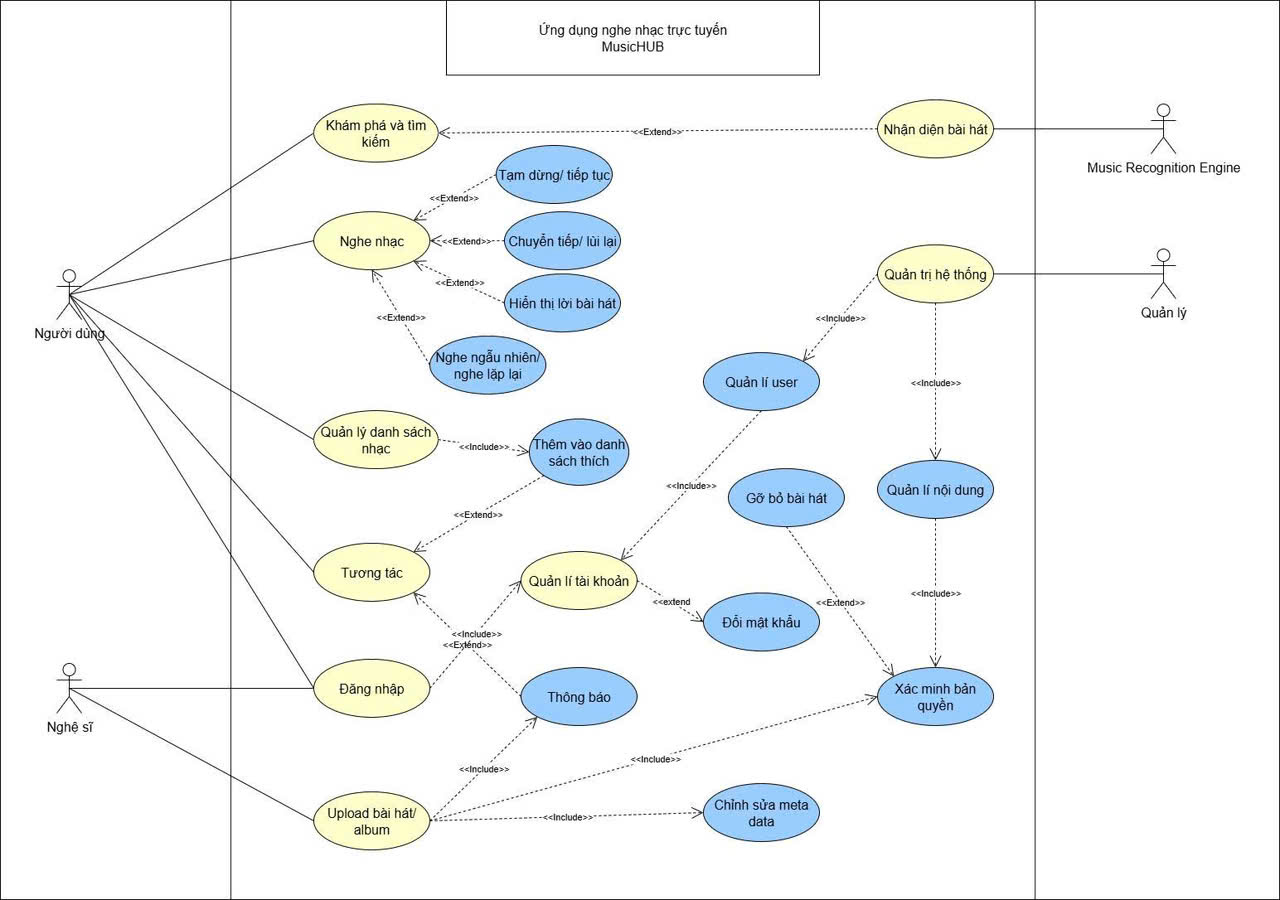
\includegraphics[width=0.9\textwidth]{Images/usecase_diagram.jpg}
	\caption{Use-case Diagram}
	\label{fig:usecase_diagram}
\end{figure}

\newpage
\subsection{Use-case Scenario}
% Upload bài hát/album - Nghệ sĩ
\subsubsection{Use-case Upload bài hát/album}
\begin{table}[H]
	\centering
	\renewcommand{\arraystretch}{1.3} % tăng khoảng cách dòng trong bảng
	\begin{tabularx}{\textwidth}{|l|X|}
		\hline
		\textbf{Use case name} & Upload bài hát/album                                                                                                                             \\ \hline
		\textbf{Actors}        & Nghệ sĩ                                                                                                                                          \\ \hline
		\textbf{Description}   & Chức năng cho phép Người dùng tải lên các bài hát của mình lên hệ thống để lưu trữ, quản lý và chia sẻ với cộng đồng nghe nhạc.                  \\ \hline
		\textbf{Trigger}       & Người dùng chọn chức năng “Upload nhạc” trên giao diện hệ thống sau khi đăng nhập thành công.                                                    \\ \hline
		\textbf{Pre-Condition(s)}
		                       & 1. Người dùng đã đăng nhập vào hệ thống. \newline
		2. Thiết bị của Người dùng được kết nối internet. \newline
		3. File nhạc đáp ứng đúng định dạng và dung lượng cho phép (ví dụ: MP3, WAV, dung lượng tối đa 20MB).                                                                     \\ \hline
		\textbf{Post-Condition(s)}
		                       & Bài hát được lưu trữ trong hệ thống, hiển thị trong thư viện cá nhân và có thể phát trực tuyến cho Người dùng khác (nếu được chia sẻ công khai). \\ \hline
		\textbf{Normal Flow}
		                       & 1. Người dùng chọn vào phần “Upload nhạc”. \newline
		2. Hệ thống hiển thị form tải nhạc (chọn file nhạc, nhập tiêu đề, Nghệ sĩ, thể loại, ảnh bìa,...). \newline
		3. Người dùng nhập thông tin và chọn file nhạc từ thiết bị. \newline
		4. Người dùng nhấn nút “Upload”. \newline
		5. Hệ thống tiến hành tải file nhạc lên server. \newline
		6. Sau khi upload thành công, hệ thống thông báo và hiển thị bài hát trong thư viện cá nhân.                                                                              \\ \hline
		\textbf{Exception Flow}
		                       & 3a. Nếu file nhạc sai định dạng hoặc vượt quá dung lượng cho phép, hệ thống thông báo lỗi. \newline
		5a. Nếu kết nối internet bị gián đoạn trong khi tải lên, hệ thống hiển thị thông báo thất bại và yêu cầu thử lại. \newline
		6a. Nếu hệ thống lỗi trong quá trình xử lý file, hiển thị thông báo “Upload thất bại”.                                                                                    \\ \hline
		\textbf{Alternative Flow}
		                       & 3b. Người dùng có thể hủy thao tác upload bất kỳ lúc nào để quay lại thư viện. \newline
		4b. Người dùng có thể chọn chế độ chia sẻ: công khai, riêng tư. \newline
		5b. Hệ thống hỗ trợ upload nhiều bài hát cùng lúc để tiết kiệm thời gian.                                                                                                 \\ \hline
	\end{tabularx}
	\caption{Mô tả use-case Upload bài hát/album}
\end{table}

% Đăng nhập & Đăng ký - Người dùng
\subsubsection{Use-case Đăng nhập \& Đăng ký}
\begin{table}[H]
	\centering
	\renewcommand{\arraystretch}{1.3} % tăng khoảng cách dòng trong bảng
	\begin{tabularx}{\textwidth}{|l|X|}
		\hline
		\textbf{Use case name} & Đăng nhập \& Đăng ký                                                                                                                                          \\ \hline
		\textbf{Actors}        & Người dùng, Nghệ sĩ                                                                                                                                           \\ \hline
		\textbf{Description}   & Người dùng có thể tạo tài khoản mới (Đăng ký) hoặc truy cập tài khoản đã có (Đăng nhập) để sử dụng ứng dụng.                                                  \\ \hline
		\textbf{Trigger}       & Người dùng mở web và chọn tính năng “Đăng nhập / Đăng ký”.                                                                                                    \\ \hline
		\textbf{Pre-Condition(s)}&
		1. Thiết bị của Người dùng phải được kết nối internet. \newline
		2. Người dùng chưa có tài khoản (nếu đăng ký) hoặc đã có tài khoản hợp lệ (nếu đăng nhập).                                                                                             \\ \hline
		\textbf{Post-Condition(s)}
		                       & Người dùng đăng nhập thành công hoặc tạo mới tài khoản thành công và được chuyển vào giao diện chính, tài khoản đăng ký thành công sẽ được thêm vào hệ thống. \\ \hline
		\textbf{Normal Flow}
		                       & \textbf{Đăng nhập:} \newline
		1. Người dùng chọn “Đăng nhập”. \newline
		2. Nhập email/số điện thoại/tên đăng nhập và mật khẩu. \newline
		3. Hệ thống kiểm tra thông tin xác thực. \newline
		4. Nếu đúng $\rightarrow$ Đăng nhập thành công và hiển thị trang chủ. \newline
		\textbf{Đăng ký:} \newline
		1. Người dùng chọn “Đăng ký”. \newline
		2. Nhập thông tin cá nhân: email/số điện thoại, mật khẩu, tên hiển thị. \newline
		3. Xác thực tài khoản qua email. \newline
		4. Hệ thống tạo tài khoản mới và hiển thị thông báo thành công.                                                                                                                        \\ \hline
		\textbf{Exception Flow}
		                       & \textbf{Đăng nhập:} \newline
		2a. Bỏ trống trường thông tin $\rightarrow$ báo lỗi “Vui lòng nhập đầy đủ thông tin”. \newline
		3a. Sai mật khẩu $\rightarrow$ báo lỗi “Sai mật khẩu”. \newline
		3b. Tài khoản bị khóa $\rightarrow$ báo lỗi “Tài khoản của bạn đã bị khóa”.
		\textbf{Đăng ký:} \newline
		2a. Email/số điện thoại đã tồn tại $\rightarrow$ báo lỗi “Tài khoản đã tồn tại”. \newline
		2b. Mật khẩu yếu/không hợp lệ $\rightarrow$ báo lỗi “Mật khẩu không hợp lệ”. \newline
		3a. Không xác thực được email $\rightarrow$ báo lỗi “Xác thực thất bại”.                                                                                                               \\ \hline
		\textbf{Alternative Flow}
		                       & \textbf{Đăng nhập:} \newline
		2b. Người Dùng chọn “Đăng nhập bằng Google/Facebook/Apple ID”. \newline
		2c. Người Dùng chọn “Quên mật khẩu” $\rightarrow$ chuyển sang luồng khôi phục mật khẩu. \newline
		\textbf{Đăng ký:} \newline
		2c. Người Dùng có thể tải ảnh đại diện hoặc chọn sở thích âm nhạc ngay khi tạo tài khoản.                                                                                              \\ \hline
	\end{tabularx}
	\caption{Mô tả use-case Đăng nhập \& Đăng ký}
\end{table}

% Quản lý tài khoản - Người dùng
\subsubsection{Use-case Quản lý tài khoản}
\begin{table}[H]
	\centering
	\renewcommand{\arraystretch}{1.3} % tăng khoảng cách dòng trong bảng
	\begin{tabularx}{\textwidth}{|l|X|}
		\hline
		\textbf{Use case name} & Quản lý tài khoản                                                                                                                                       \\ \hline
		\textbf{Actors}        & Người dùng, Nghệ sĩ                                                                                                                                     \\ \hline
		\textbf{Description}   & Người dùng có thể quản lý tài khoản cá nhân bao gồm: đăng ký, đổi mật khẩu, cập nhật thông tin cá nhân (avatar, tên hiển thị, email), và xóa tài khoản. \\ \hline
		\textbf{Trigger}       & Người dùng chọn chức năng “Quản lý tài khoản” trên giao diện hệ thống sau khi đăng nhập thành công.                                                     \\ \hline
		\textbf{Pre-Condition(s)}
		                       & 1. Thiết bị của Người dùng phải được kết nối internet. \newline
		2. Người dùng đã đăng nhập thành công.                                                                                                                                           \\ \hline
		\textbf{Post-Condition(s)}
		                       & Hệ thống cập nhật thông tin tài khoản theo thao tác của Người Dùng.                                                                                     \\ \hline
		\textbf{Normal Flow}
		                       & 1. Người dùng chọn vào phần “Quản lý tài khoản” trong giao diện hệ thống. \newline
		2. Hệ thống hiển thị thông tin tài khoản hiện tại. \newline
		3. Người dùng chọn hành động: chỉnh sửa thông tin cá nhân / đổi mật khẩu / thiết lập bảo mật. \newline
		4. Người dùng nhập thông tin mới hoặc thay đổi cần thiết. \newline
		5. Người dùng xác nhận và lưu thay đổi. \newline
		6. Hệ thống cập nhật dữ liệu và thông báo thành công.                                                                                                                            \\ \hline
		\textbf{Exception Flow}
		                       & 3a. Nếu hệ thống không tải được thông tin tài khoản thì hiển thị lỗi “Không thể tải dữ liệu”. \newline
		4a. Nếu thông tin nhập sai định dạng (ví dụ email không hợp lệ, mật khẩu quá ngắn), hệ thống thông báo lỗi và yêu cầu nhập lại. \newline
		5a. Nếu kết nối internet bị gián đoạn trong khi lưu, hệ thống hiển thị thông báo thất bại và yêu cầu thử lại.                                                                    \\ \hline
		\textbf{Alternative Flow}
		                       & 3b. Người dùng có thể hủy thao tác và quay lại trang chính mà không thay đổi gì. \newline
		4b. Người dùng có thể bật/tắt các tính năng nâng cao như xác thực 2 lớp.                                                                                                         \\ \hline
	\end{tabularx}
	\caption{Mô tả use-case Quản lý tài khoản}
\end{table}

% Tương tác - Người dùng
\subsubsection{Use-case Tương tác}
\begin{table}[H]
	\centering
	\renewcommand{\arraystretch}{1.3} % tăng khoảng cách dòng trong bảng
	\begin{tabularx}{\textwidth}{|l|X|}
		\hline
		\textbf{Use case name} & Tương tác                                                                                                                                                                              \\ \hline
		\textbf{Actors}        & Người dùng                                                                                                                                                                             \\ \hline
		\textbf{Description}   & Người dùng có thể thực hiện các hành động tương tác trong hệ thống như: thích (like) bài hát, bình luận bài hát, theo dõi nghệ sĩ, chia sẻ bài hát, nghệ sĩ, playlist lên mạng xã hội. \\ \hline
		\textbf{Trigger}       & Người dùng chọn một bài hát, nghệ sĩ hoặc playlist bất kỳ trong hệ thống và mở giao diện chi tiết.                                                                                     \\ \hline
		\textbf{Pre-Condition(s)}
		                       & 1. Thiết bị của Người dùng phải được kết nối internet. \newline
		2. Người dùng đã đăng nhập thành công. \newline
		3. Bài hát, nghệ sĩ đã có sẵn trên hệ thống.                                                                                                                                                                    \\ \hline
		\textbf{Post-Condition(s)}
		                       & Hệ thống lưu lại thông tin tương tác (like, bình luận, theo dõi, chia sẻ) và cập nhật dữ liệu liên quan.                                                                               \\ \hline
		\textbf{Normal Flow}
		                       & 1. Người dùng chọn một bài hát, nghệ sĩ, playlist. \newline
		2. Hệ thống hiển thị chi tiết bài hát, nghệ sĩ, playlist. \newline
		3. Người dùng chọn hành động muốn thực hiện: \newline
		\cach 3a. Nhấn nút “Thích” (Like) để thêm vào danh sách yêu thích. \newline
		\cach 3b. Viết và gửi bình luận cho bài hát. \newline
		\cach 3c. Nhấn “Theo dõi” để theo dõi nghệ sĩ. \newline
		\cach 3d. Chọn “Chia sẻ” và lựa chọn kênh chia sẻ (Các trang mạng xã \cach hội). \newline
		4. Hệ thống xác nhận và cập nhật thông tin tương tác.                                                                                                                                                           \\ \hline
		\textbf{Exception Flow}
		                       & 2a. Nếu bài hát, nghệ sĩ, playlist không tồn tại hoặc bị xóa $\rightarrow$ hiển thị thông báo lỗi. \newline
		3b1. Nếu bình luận chứa nội dung vi phạm chính sách $\rightarrow$ hệ thống từ chối đăng và hiển thị thông báo. \newline
		3d1. Nếu chia sẻ thất bại do mất kết nối internet $\rightarrow$ hiển thị thông báo “Chia sẻ không thành công, vui lòng thử lại”.                                                                                \\ \hline
		\textbf{Alternative Flow}
		                       & 3a1. Người dùng có thể “Bỏ thích” (Unlike) nếu trước đó đã thích. \newline
		3b2. Người dùng có thể chỉnh sửa hoặc xóa bình luận đã đăng. \newline
		3c1. Người dùng có thể hủy theo dõi nghệ sĩ. \newline
		3d2. Người dùng có thể sao chép đường dẫn (link) thay vì chia sẻ trực tiếp.                                                                                                                                     \\ \hline
	\end{tabularx}
	\caption{Mô tả use-case Tương tác}
\end{table}

% Nghe nhạc - Người dùng
\subsubsection{Use-case Nghe nhạc}
\begin{table}[H]
	\centering
	\renewcommand{\arraystretch}{1.3} % tăng khoảng cách dòng trong bảng
	\begin{tabularx}{\textwidth}{|l|X|}
		\hline
		\textbf{Use case name} & Nghe nhạc                                                                                                                                                                                                                                                                   \\ \hline
		\textbf{Actors}        & Người dùng                                                                                                                                                                                                                                                                  \\ \hline
		\textbf{Description}   & Người dùng có thể phát và điều khiển nhạc với nhiều tính năng nâng cao: phát/tạm dừng, tiếp tục, chuyển tiếp/lùi lại, bật chế độ nghe ngẫu nhiên, nghe lặp lại (một bài hoặc toàn bộ danh sách), thêm bài vào hàng chờ, cài giờ tắt nhạc (sleep timer), và xem lời bài hát. \\ \hline
		\textbf{Trigger}       & Người dùng chọn một bài hát, playlist, album và nhấn nút “Phát nhạc”.                                                                                                                                                                                                       \\ \hline
		\textbf{Pre-Condition(s)}
		                       & 1. Thiết bị của Người dùng phải được kết nối internet. \newline
		2. Ứng dụng được cấp quyền truy cập âm thanh. \newline
		3. Người dùng đã đăng nhập thành công. \newline
		4. Bài hát đã có sẵn trên hệ thống và có thể phát.                                                                                                                                                                                                                                                   \\ \hline
		\textbf{Post-Condition(s)}
		                       & Hệ thống phát nhạc theo thao tác của Người dùng, cập nhật trạng thái trình phát (player state) và lưu lại lịch sử nghe nhạc.                                                                                                                                                \\ \hline
		\textbf{Normal Flow}
		                       & 1. Người dùng chọn một bài hát, playlist, album. \newline
		2. Hệ thống tải dữ liệu nhạc và bắt đầu phát. \newline
		3. Người dùng có thể thực hiện các thao tác điều khiển: \newline
		\cach 3a. Nhấn “Tạm dừng” (Pause) hoặc “Tiếp tục” (Play). \newline
		\cach 3b. Nhấn “Chuyển tiếp” (Next) hoặc “Lùi lại” (Previous). \newline
		\cach 3c. Bật chế độ “Nghe ngẫu nhiên” (Shuffle). \newline
		\cach 3d. Chọn chế độ “Nghe lặp lại” (Repeat one / Repeat all). \newline
		\cach 3e. Thêm bài hát vào hàng chờ phát (Queue). \newline
		\cach 3f. Cài đặt “Giờ tắt nhạc” (Sleep timer). \newline
		\cach 3g. Xem lời bài hát (Lyrics) nếu có sẵn. \newline
		4. Hệ thống phản hồi ngay lập tức và cập nhật trình phát nhạc. \newline
		5. Khi bài hát kết thúc, hệ thống tự động phát bài tiếp theo trong playlist/queue hoặc dừng lại nếu không còn bài nào                                                                                                                                                                                \\ \hline
		\textbf{Exception Flow}
		                       & 2a. Nếu bài hát không thể phát (do bản quyền hoặc lỗi file) $\rightarrow$  hiển thị thông báo. \newline
		2b. Nếu người dùng bị mất kết nối trong lúc đang phát nhạc $\rightarrow$ hiển thị thông báo “Mất kết nối, vui lòng kiểm tra lại” và tạm dừng phát nhạc. \newline
		3g1. Nếu bài hát không có lời (lyrics) trong cơ sở dữ liệu $\rightarrow$ hiển thị “Chưa có lời bài hát”.                                                                                                                                                                                             \\ \hline
		\textbf{Alternative Flow}
		                       & 3a1. Người dùng có thể sử dụng tai nghe hoặc thiết bị ngoài để điều khiển (nút Play/Pause). \newline
		3e1. Người dùng có thể sắp xếp lại thứ tự bài hát trong hàng chờ. \newline
		3f2. Người dùng có thể hủy hoặc thay đổi thời gian sleep timer.                                                                                                                                                                                                                                      \\ \hline
	\end{tabularx}
	\caption{Mô tả use-case Nghe nhạc}
\end{table}

% Khám phá và tìm kiếm - Người dùng
\subsubsection{Use-case Khám phá và tìm kiếm}
\begin{table}[H]
	\centering
	\renewcommand{\arraystretch}{1.3} % tăng khoảng cách dòng trong bảng
	\begin{tabularx}{\textwidth}{|l|X|}
		\hline
		\textbf{Use case name} & Khám phá và tìm kiếm                                                                                                                                 \\ \hline
		\textbf{Actors}        & Người dùng                                                                                                                                           \\ \hline
		\textbf{Description}   & Người dùng có thể tìm kiếm bài hát, nghệ sĩ, album, playlist và khám phá nhạc mới thông qua bảng xếp hạng, xu hướng (trending) và gợi ý cá nhân hóa. \\ \hline
		\textbf{Trigger}       & Người dùng mở thanh tìm kiếm hoặc tab “Khám phá” trong ứng dụng.                                                                                     \\ \hline
		\textbf{Pre-Condition(s)}
		                       & 1. Thiết bị của Người dùng phải được kết nối internet. \newline
		2. Người dùng đã đăng nhập thành công. \newline 
		3. Dữ liệu về bài hát, nghệ sĩ, album phải có trong cơ sở dữ liệu.                                                                                                            \\ \hline
		\textbf{Post-Condition(s)}
		                       & Hệ thống trả về kết quả tìm kiếm hoặc danh sách nhạc khám phá phù hợp, cho phép Người dùng chọn và nghe nhạc ngay.                                   \\ \hline
		\textbf{Normal Flow}
		                       & 1. Người dùng mở tính năng Tìm kiếm/Khám phá. \newline
		2. Người dùng có thể thực hiện: \newline
		\cach 2a. Nhập từ khóa để tìm bài hát, nghệ sĩ, album, playlist. \newline
		\cach 2b. Xem danh sách Trending hoặc Top Chart. \newline
		\cach 2c. Nhận gợi ý nhạc cá nhân hóa dựa trên lịch sử nghe, lượt thích và nghệ sĩ theo dõi. \newline
		3. Hệ thống hiển thị danh sách kết quả. \newline
		4. Người dùng chọn nội dung mong muốn (phát nhạc, xem chi tiết nghệ sĩ, album, playlist).                                                                                     \\ \hline
		\textbf{Exception Flow}
		                       & 2a1. Nếu không tìm thấy kết quả $\rightarrow$ hiển thị thông báo “Không tìm thấy nội dung phù hợp”. \newline
		2a2. Nếu không nhập gì $\rightarrow$ hiển thị “Vui lòng nhập từ khóa”. \newline
		2a3. Nếu kết nối internet bị gián đoạn trong khi tìm kiếm $\rightarrow$ hiển thị thông báo “Mất kết nối, vui lòng kiểm tra lại”.											  \\ \hline
		\textbf{Alternative Flow}
		                       & 2a2. Người dùng có thể dùng bộ lọc nâng cao (theo thể loại, năm phát hành, nghệ sĩ, album…). \newline
		2b2. Người dùng có thể chọn xem bảng xếp hạng theo từng khu vực/quốc gia. \newline
		2c2. Người dùng có thể cập nhật gợi ý bằng cách thay đổi sở thích cá nhân (genres, mood…).                                                                                    \\ \hline
	\end{tabularx}
	\caption{Mô tả use-case Khám phá và tìm kiếm}
\end{table}

% Nhận diện bài hát - Người dùng
\subsubsection{Use-case Nhận diện bài hát}
\begin{table}[H]
	\centering
	\renewcommand{\arraystretch}{1.3} % tăng khoảng cách dòng trong bảng
	\begin{tabularx}{\textwidth}{|l|X|}
		\hline
		\textbf{Use case name} & Nhận diện bài hát                                                                                                                                                  \\ \hline
		\textbf{Actors}        & Người dùng                                                                                                                                                         \\ \hline
		\textbf{Description}   & Người dùng bật tính năng nhận diện nhạc để hệ thống nghe một đoạn nhạc từ môi trường xung quanh, sau đó so sánh với cơ sở dữ liệu fingerprint để xác định bài hát. \\ \hline
		\textbf{Trigger}       & Người dùng nhấn vào biểu tượng "Nhận diện bài hát" trên thanh tìm kiếm.                                                                                            \\ \hline
		\textbf{Pre-Condition(s)}
		                       & 1. Thiết bị của Người dùng phải được kết nối internet. \newline
		2. Ứng dụng được cấp quyền truy cập micro. \newline
		3. Hệ thống có cơ sở dữ liệu nhạc đủ lớn để so khớp.                                                                                                                                        \\ \hline
		\textbf{Post-Condition(s)}
		                       & Hệ thống hiển thị thông tin bài hát (tên, nghệ sĩ, album) và cung cấp tùy chọn phát nhạc hoặc lưu vào playlist.                                                    \\ \hline
		\textbf{Normal Flow}
		                       & 1. Người dùng chọn tính năng Nhận diện bài hát. \newline
		2. Hệ thống yêu cầu quyền truy cập micro và người dùng cấp phép. \newline
		3. Hệ thống ghi lại một đoạn âm thanh từ 15-20s. \newline
		4. Hệ thống trích xuất "Fingerprint" (dấu vân tay âm thanh) từ đoạn ghi âm để so khớp với dữ liệu. \newline
		5. Hệ thống trả về kết quả gồm tên bài hát, nghệ sĩ, album (nếu có). \newline
		6. Người dùng có thể chọn nghe bài hát, thêm vài playlist hoặc chia sẻ.                                                                                                                     \\ \hline
		\textbf{Exception Flow}
		                       & 2a. Người dùng từ chối quyền micro $\rightarrow$ hệ thống báo không thể sử dụng tính năng. \newline
		3a. Không thu được âm thanh do quá ồn, micro hỏng $\rightarrow$ hệ thống yêu cầu thử lại. \newline
		5a. Nếu không tìm thấy kết quả khớp $\rightarrow$ hệ thống thông báo “Không nhận diện được bài hát”. \newline
		5b. Nếu có lỗi kết nối trong quá trình so khớp $\rightarrow$ hệ thống báo “Mất kết nối” và cho phép thử lại sau.                                                                            \\ \hline
		\textbf{Alternative Flow}
		                       & 5c. Người dùng có thể tìm kiếm bài hát thủ công.                                                                                                                   \\ \hline
	\end{tabularx}
	\caption{Mô tả use-case Nhận diện bài hát}
\end{table}

% Quản lý danh sách nhạc - Người dùng
\subsubsection{Use-case Quản lý danh sách nhạc}
\begin{table}[H]
	\centering
	\renewcommand{\arraystretch}{1.3} % tăng khoảng cách dòng trong bảng
	\begin{tabularx}{\textwidth}{|l|X|}
		\hline
		\textbf{Use case name} & Quản lý danh sách nhạc                                                                                                                                                             \\ \hline
		\textbf{Actors}        & Người dùng                                                                                                                                                                         \\ \hline
		\textbf{Description}   & Cho phép người dùng xem, thêm, sửa và xóa bài hát trong danh sách nhạc của họ.                                                                                                     \\ \hline
		\textbf{Trigger}       & Người dùng truy cập danh sách nhạc và chọn một chức năng quản lý danh sách nhạc (tạo danh sách, thêm bài hát, xóa bài hát, xóa danh sách, .v.v).                                   \\ \hline
		\textbf{Pre-Condition(s)}
		                       & 1. Thiết bị của Người dùng phải được kết nối internet. \newline
		2. Người dùng đã đăng nhập thành công. \newline
		3. Hệ thống có ít nhất một bài hát.                                                                                                                                                                         \\ \hline
		\textbf{Post-Condition(s)}
		                       & 1. Danh sách nhạc của User được cập nhật theo hành động đã thực hiện (thêm, sửa, xóa). \newline
		2. Người dùng nhận được thông báo về kết quả của hành động.                                                                                                                                                 \\ \hline
		\textbf{Normal Flow}
		                       & 1. Người dùng truy cập vào phần “Danh sách nhạc của tôi” trong giao diện hệ thống. \newline
		2. Hệ thống hiển thị danh sách nhạc của người dùng hiện tại. \newline
		3. Người dùng thực hiện thao tác điều khiển: \newline
		\cach 3a. Người dụng chọn ``Tạo playlist mới'', hệ thống hiển thị yêu cầu điền tên playlist, người dùng nhập và nhấn xác nhận. \newline
		\cach 3b. Người dùng chọn ``Thêm vào playlist'' với bài hát muốn thêm, hệ thống yêu cầu chọn playlist muốn thêm, người dùng chọn và nhấn xác nhận. \newline
		\cach 3c. Người dùng chọn ``Xóa khỏi playlist'' với bài hát muốn xóa, hệ thống hiển thị thông báo xác nhận, người dùng xác nhận. \newline
		\cach 3d. Người dùng chọn ``Xóa playlist'', hệ thống hiển thị thông báo xác nhận, người dùng xác nhận. \newline
		4. Hệ thống ghi nhận và cập nhật danh sách playlist của người dùng.                                                                                                                                         \\ \hline
		\textbf{Exception Flow}
		                       & 1. Nếu lỗi xảy ra (mất kết nối máy chủ, hệ thống bận, .v.v), mọi yêu cầu từ người dùng đều bị từ chối và hệ thống sẽ hiển thị thông báo ``Đang trong quá trình bảo trì''. \newline
		3a. Nếu người dùng nhập tên playlist đã tồn tại, hệ thống thông báo lỗi và yêu cầu người dùng nhập lại. \newline
		3b. Nếu người dùng thêm 1 bài hát đã tồn tại trong playlist, hệ thống hiển thị thông báo đã tồn tại và không cập nhật bài hát.                                                                              \\ \hline
		\textbf{Alternative Flow}
		                       & 3a. Người dùng không đặt tên mà trực tiếp xác nhận, hệ thống vẫn sẽ ghi nhận và đặt tên theo format mặc định ``Unnamed Playlist''.\newline
		3c/3d. Nếu người dùng không xác nhận, hệ thống hoàn tác toàn bộ thao tác và cập nhật lại trạng thái ban đầu của danh sách playlist.                                                                         \\ \hline
	\end{tabularx}
	\caption{Mô tả use-case Quản lý danh sách nhạc}
\end{table}

% Quản trị hệ thống - Quản lý
\subsubsection{Use-case Quản trị hệ thống}
\begin{table}[H]
	\centering
	\renewcommand{\arraystretch}{1.3} % tăng khoảng cách dòng trong bảng
	\begin{tabularx}{\textwidth}{|l|X|}
		\hline
		\textbf{Use case name} & Quản trị hệ thống                                                                                                                                                                                                  \\ \hline
		\textbf{Actors}        & Quản lý                                                                                                                                                                                                            \\ \hline
		\textbf{Description}   & Cho phép quản lý thực hiện các tác vụ quản trị để duy trì và điều hành hệ thống.                                                                                                                                   \\ \hline
		\textbf{Trigger}       & Quản lý truy cập vào trang quản lý hệ thống trong giao diện quản lý.                                                                                                                                               \\ \hline
		\textbf{Pre-Condition(s)}
		                       & 1. Thiết bị của quản lý phải được kết nối internet. \newline
		2. Quản lý đã đăng nhập thành công \textbf{dưới quyền quản trị}.                                                                                                                                                                            \\ \hline
		\textbf{Post-Condition(s)}
		                       & 1. Các thay đổi về người dùng, nội dung, hoặc bản quyền đã được cập nhật thành công trong hệ thống. \newline
		2. Hệ thống duy trì trạng thái ổn định và các quy định được tuân thủ.                                                                                                                                                                       \\ \hline
		\textbf{Normal Flow}
		                       & 1. Quản lý truy cập vào trang quản lý hệ thống với tài khoản có quyền quản trị. \newline
		2. Hệ thống điều hướng đến trang quản trị hệ thống. \newline
		3. Quản lý có thể lựa chọn hành động: \newline
		\cach 3a. Xem, sửa (đối với quyền truy cập), xóa người dùng. \newline
		\cach 3b. Phê duyệt, gỡ bỏ nội dung, bài hát, album công khai thủ công. \newline
		\cach 3c. Thay đổi các thông tin của nội dung phù hợp với chính sách. \newline
		\cach 3d. Kiểm tra tính minh bạch và bản quyền của nội dung đăng tải. \newline
		4. Hệ thống thông báo thao tác thành công. \newline
		5. Hệ thống tự động ghi log đảm bảo tính minh bạch về sau.                                                                                                                                                                                  \\ \hline
		\textbf{Exception Flow}
		                       & 3.1. Nếu quản lý cố gắng truy cập một chức năng không có quyền, hệ thống sẽ thông báo lỗi ``Bạn không có quyền truy cập chức năng này''. \newline
		3.2. Nếu có lỗi trong quá trình cập nhật dữ liệu (thông tin không hợp lệ, .v.v), hệ thống sẽ hiển thị thông báo lỗi và không thực hiện thay đổi. \newline
		3.3. Nếu lỗi xảy ra (mất kết nối máy chủ, hệ thống bận, .v.v), mọi thông tin thay đổi sẽ được lưu tạm thời và hệ thống sẽ hiển thị thông báo ``Đang trong quá trình bảo trì'' cho tới khi có kết nối lại và tự động thực hiện lại thao tác. \\ \hline
		\textbf{Alternative Flow}
		                       & 1a. Tài khoản không có quyền thì hệ thống tự động điều hướng đến giao diện người dùng bình thường. \newline
		3a/3b/3c/3d. Nếu thao tác không được xác nhận, hệ thống hoàn tác toàn bộ thao tác và cập nhật lại trạng thái ban đầu của nội dung.                                                                                                          \\ \hline
	\end{tabularx}
	\caption{Mô tả use-case Quản trị hệ thống}
\end{table}
% Thiết kế hành vi và giao diện người dùng
\newpage
\section{Thiết kế hành vi và giao diện người dùng}
% Đăng nhập - đăng kí
\subsection{Đăng nhập - đăng kí}
% Đăng nhập - Người dùng
\subsubsection{Đăng nhập - Login}
\begin{itemize}
	\item \textbf{Sequence Diagram:}
	      \begin{figure}[H]
		      \centering
		      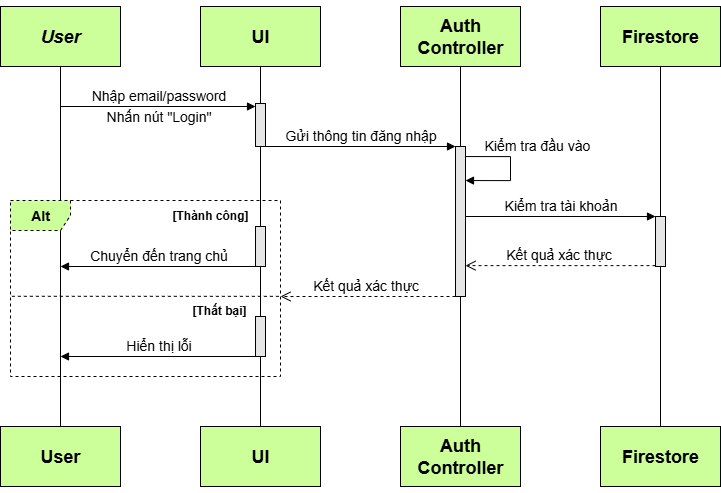
\includegraphics[width=0.9\textwidth]{Images/login_sequence.png}
		      \caption{Sequence Diagram - Login}
	      \end{figure}
	\item \textbf{Mục đích:} Thể hiện quy trình đăng nhập của người dùng, bao gồm các bước từ khi người dùng nhập thông tin đến khi hệ thống xác thực và phản hồi kết quả.
	\item \textbf{Thành phần liên quan:}
	      \begin{itemize}
		      \item Người dùng (User): người thực hiện thao tác đăng nhập.
		      \item Giao diện đăng nhập (Login UI): giao diện để người dùng nhập thông tin và hiển thị kết quả.
		      \item Hệ thống xác thực (Auth Controller): nhận thông tin đăng nhập và xử lý xác thực.
		      \item Cơ sở dữ liệu người dùng (Firestore): lưu trữ thông tin tài khoản.
	      \end{itemize}
	\item \textbf{Luồng tương tác:}
	      \begin{enumerate}
		      \item Người dùng mở trang đăng nhập.
		      \item Người dùng nhập email + mật khẩu và nhấn nút “Đăng nhập”.
		      \item Giao diện đăng nhập gửi yêu cầu đăng nhập đến Hệ thống xác thực.
		      \item Hệ thống xác thực kiểm tra dữ liệu đầu vào (có trống không, định dạng hợp lệ không).
		      \item Nếu hợp lệ, Hệ thống xác thực truy vấn Cơ sở dữ liệu người dùng để tìm tài khoản.
		      \item Cơ sở dữ liệu trả về thông tin tài khoản (nếu tồn tại).
		      \item Hệ thống xác thực phản hồi lại cho Giao diện đăng nhập:
		            \begin{itemize}
			            \item Nếu đúng: thông báo đăng nhập thành công và chuyển đến giao diện trang chủ.
			            \item Nếu sai: thông báo lỗi (sai mật khẩu, tài khoản không tồn tại).
		            \end{itemize}
	      \end{enumerate}
	\item \textbf{Activity Diagram:}
	      \begin{figure}[H]
		      \centering
		      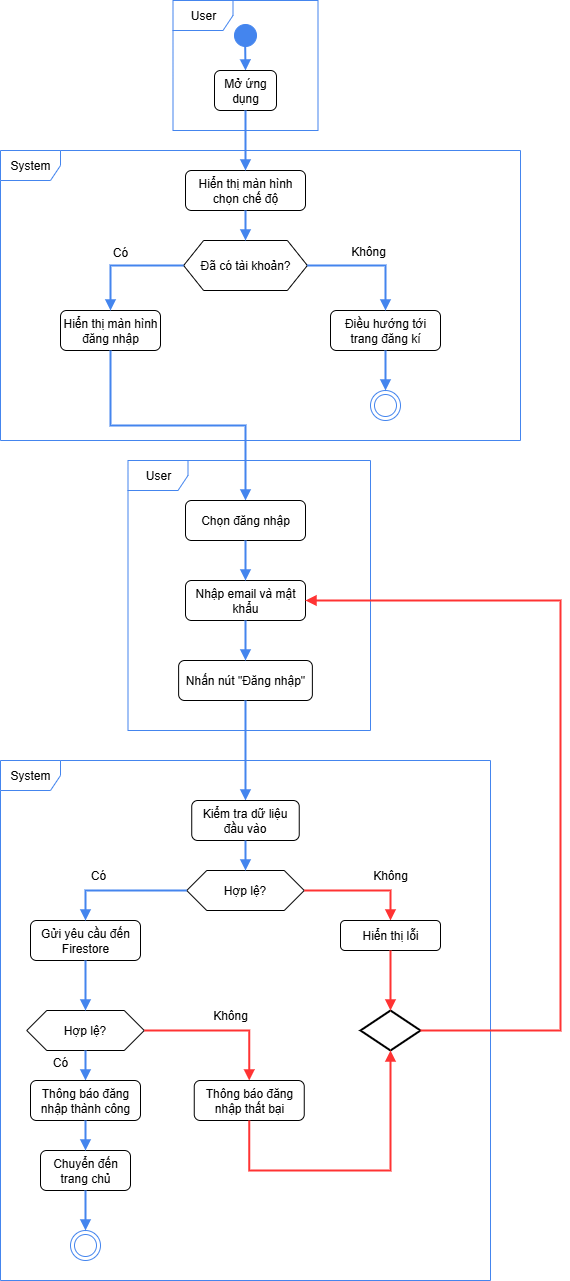
\includegraphics[width=0.6\textwidth]{Images/login_activity.png}
		      \caption{Activity Diagram - Login}
	      \end{figure}
	\item \textbf{UI:}
\end{itemize}
% Đăng ký - Người dùng
\subsubsection{Đăng ký - Register}
\begin{itemize}
	\item \textbf{Sequence Diagram:}
	      \begin{figure}[H]
		      \centering
		      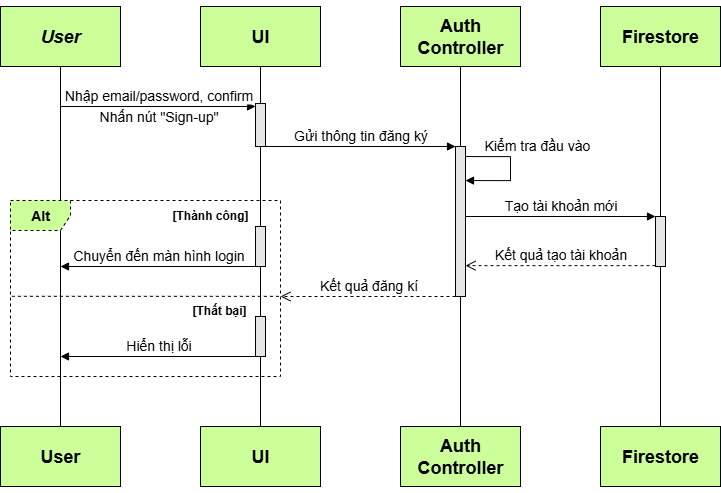
\includegraphics[width=0.9\textwidth]{Images/register_sequence.png}
		      \caption{Sequence Diagram - Register}
	      \end{figure}
	\item \textbf{Mục đích:} Thể hiện quy trình đăng ký tài khoản mới của người dùng, bao gồm các bước từ khi người dùng nhập thông tin đến khi hệ thống tạo tài khoản và phản hồi kết quả.
	\item \textbf{Thành phần liên quan:}
	      \begin{itemize}
		      \item Người dùng (User): người thực hiện thao tác đăng ký.
		      \item Giao diện đăng ký (Register UI): giao diện để người dùng nhập thông tin và hiển thị kết quả.
		      \item Hệ thống xác thực (Auth Controller): nhận thông tin đăng ký và xử lý xác thực.
		      \item Cơ sở dữ liệu người dùng (Firestore): lưu trữ thông tin tài khoản.
	      \end{itemize}
	\item \textbf{Luồng tương tác:}
	      \begin{enumerate}
		      \item Người dùng mở trang đăng ký.
		      \item Người dùng nhập email, mật khẩu và xác nhận mật khẩu, sau đó nhấn nút “Đăng ký”.
		      \item Giao diện đăng ký gửi yêu cầu tạo tài khoản đến Hệ thống xác thực.
		      \item Hệ thống xác thực kiểm tra dữ liệu đầu vào (có trống không, mật khẩu có khớp không, định dạng email hợp lệ không).
		      \item Nếu hợp lệ, Hệ thống xác thực truy vấn Cơ sở dữ liệu người dùng để kiểm tra xem tài khoản đã tồn tại hay chưa.
		      \item Cơ sở dữ liệu phản hồi kết quả kiểm tra.
		      \item Hệ thống xác thực phản hồi lại cho Giao diện đăng ký:
		            \begin{itemize}
			            \item Nếu tài khoản chưa tồn tại: tạo tài khoản mới, thông báo đăng ký thành công và điều hướng người dùng đến giao diện đăng nhập.
			            \item Nếu tài khoản đã tồn tại hoặc dữ liệu không hợp lệ: thông báo lỗi (email đã tồn tại, mật khẩu không khớp, định dạng sai, v.v.).
		            \end{itemize}
	      \end{enumerate}

	\item \textbf{Activity Diagram:}
	      \begin{figure}[H]
		      \centering
		      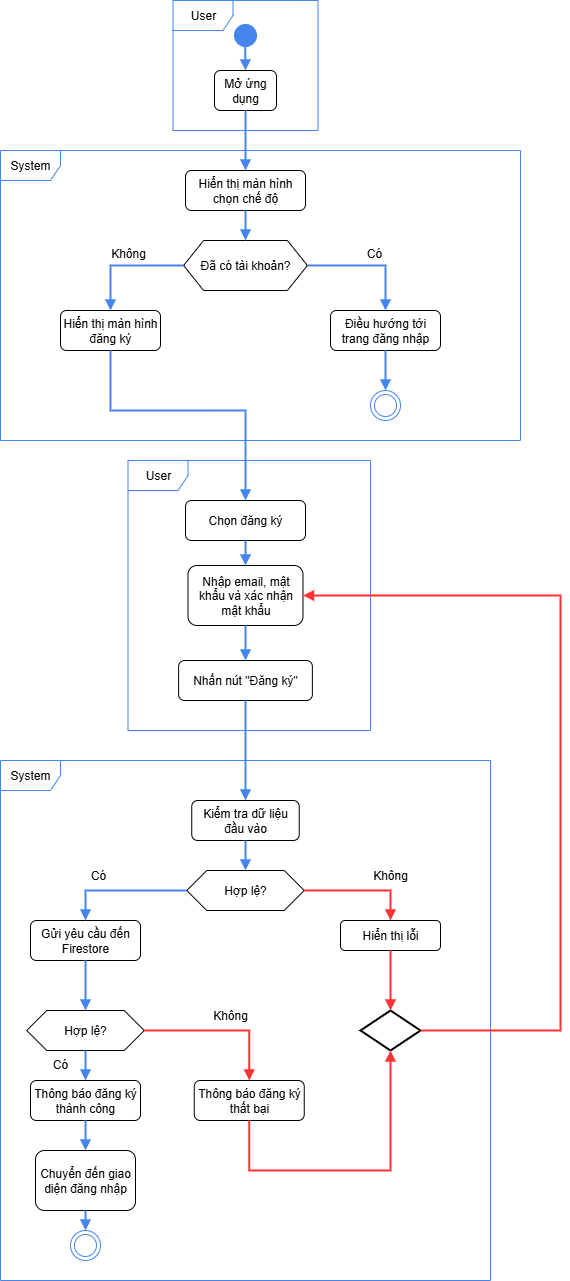
\includegraphics[width=0.6\textwidth]{Images/register_activity.png}
		      \caption{Activity Diagram - Register}
	      \end{figure}
	\item \textbf{UI:}


\end{itemize}
% Quản lý tài khoản - Người dùng
\subsection{Quản lý tài khoản - Account Management}
\begin{itemize}
	\item \textbf{Sequence Diagram:}
	      \begin{figure}[H]
		      \centering
		      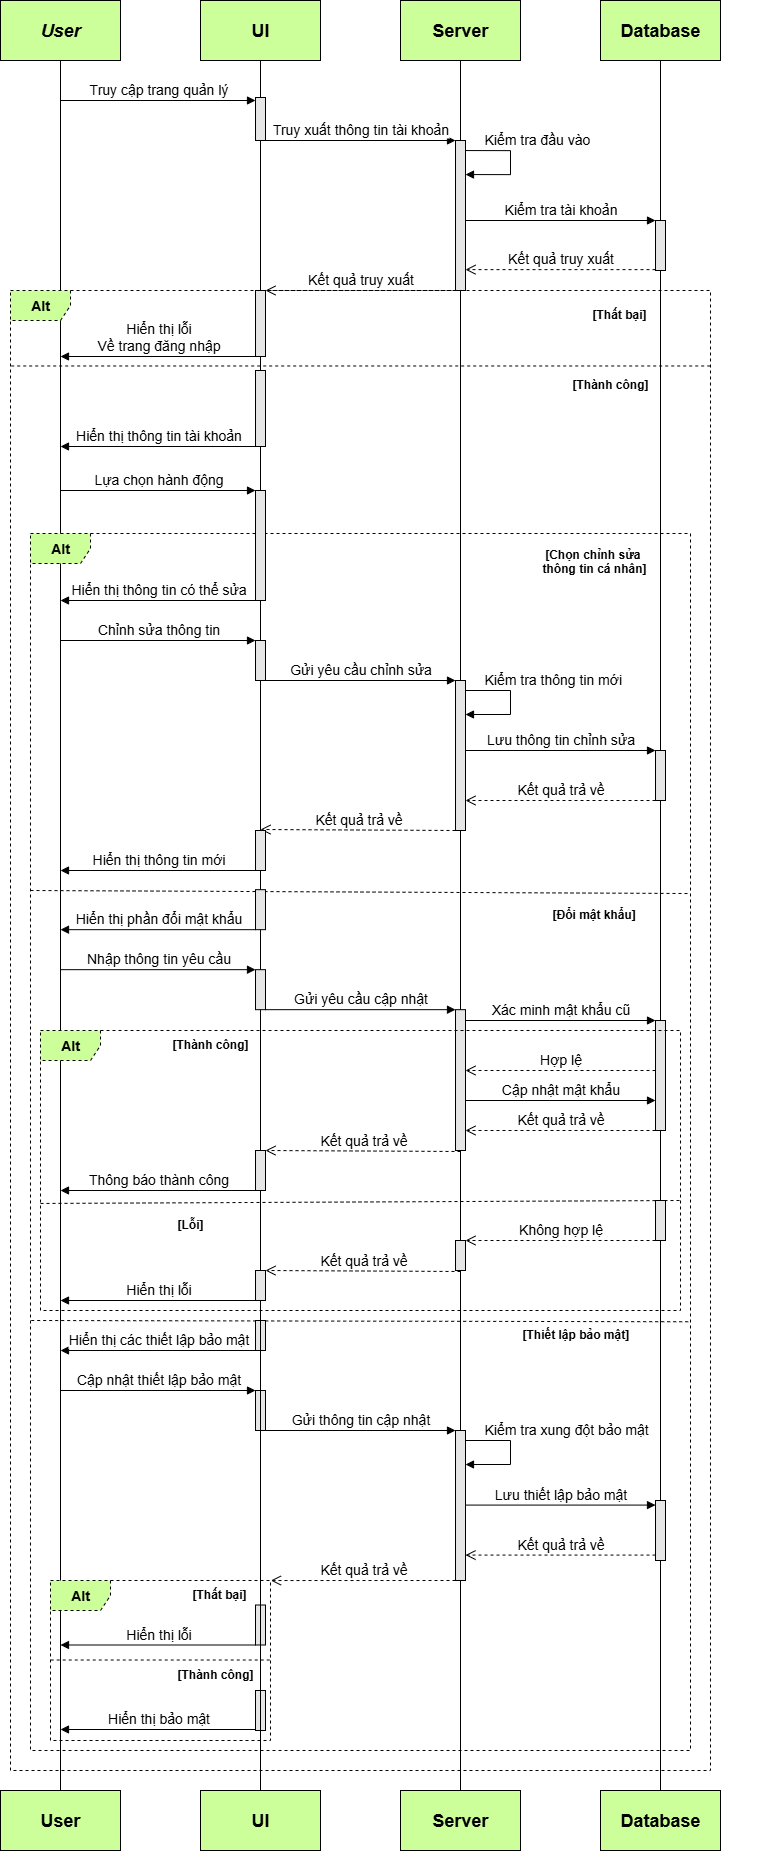
\includegraphics[width=0.5\textwidth]{Images/account-management_sequence.png}
		      \caption{Sequence Diagram - Account Management}
	      \end{figure}
	\item \textbf{Mục đích:} Thể hiện các tùy chọn quản lý tài khoản cho người dùng.
	\item \textbf{Thành phần liên quan:}
	      \begin{itemize}
		      \item Người dùng (User): người thực hiện thao tác đăng ký.
		      \item Giao diện quản lý (Management UI): giao diện để người dùng nhập thông tin và hiển thị kết quả.
		      \item Hệ thống xử lý (Server): nhận thông tin xác thực dữ liệu.
		      \item Cơ sở dữ liệu người dùng (Database): lưu trữ thông tin tài khoản.
	      \end{itemize}
	\item \textbf{Luồng tương tác:}
	      \begin{enumerate}
		      \item Người dùng mở trang quản lý tài khoản.
		      \item Hệ thống xử lý gửi yêu cầu đến cơ sở dữ liệu.
		      \item Cơ sở dữ liệu phản hồi kết quả kiểm tra.
		      \item Hệ thống kiểm tra trạng thái tài khoản, nếu chưa hợp lệ, thông báo lỗi và điều hướng về trang đăng nhập.
		      \item Nếu hợp lệ, hệ thống trả về thông tin tài khoản và hiển thị lên giao diện.
		      \item Người dụng lựa chọn chức năng:
		            \begin{itemize}
			            \item Nếu người dùng chọn chỉnh sửa thông tin tài khoản:
			                  \begin{itemize}
				                  \item Giao diện hiển thị thông tin tài khoản có thể chỉnh sửa.
				                  \item Người dùng tiến hành chỉnh sửa và xác nhận.
				                  \item Hệ thống tiếp nhận yêu cầu sửa chữa và kiểm tra tính đúng đắn của dữ liệu.
				                  \item Nếu thông tin hợp lệ, hệ thống gửi yêu cầu cập nhật dữ liệu đến cơ sở dữ liệu.
				                  \item Cơ sở dữ liệu cập nhật dữ liệu mới và phản hồi nội dung cập nhật.
				                  \item Hệ thống gửi trả nội dung mới.
				                  \item Giao diện cập nhật theo nội dung mới của người dùng.
			                  \end{itemize}
			            \item Nếu người dùng chọn đổi mật khẩu:
			                  \begin{itemize}
				                  \item Giao diện hiển thị biểu mẫu nhập mật khẩu cũ và mật khẩu mới.
				                  \item Người dùng nhập dữ liệu theo yêu cầu và xác nhận.
				                  \item Hệ thống tiếp nhận mật khẩu cũ và gửi đến cơ sở dữ liệu kiểm tra hợp lệ.
				                  \item Cơ sở dữ liệu phản hồi kết quả.
				                  \item Nếu dữ liệu hợp lệ, hệ thống gửi thông tin mật khẩu mới đến cơ sở dữ liệu.
				                  \item Cơ sở dữ liệu cập nhật mật khẩu mới và phản hồi nội dung cập nhật.
				                  \item Hệ thống gửi trả phản hồi thành công.
				                  \item Giao diện thông báo cập nhật thành công.
			                  \end{itemize}
			            \item Nếu người dùng chọn thiết lập bảo mật:
			                  \begin{itemize}
				                  \item Giao diện hiển thị các thiết lập bảo mật.
                          \item Người dùng xác nhận các thiết lập bảo mật.
                          \item Hệ thống tiếp nhận và gửi yêu cầu đến cơ sở dữ liệu.
                          \item Cơ sở dữ liệu cập nhật và phản hồi nội dung cập nhật.
                          \item Hệ thống gửi trả phản hồi thành công.
                          \item Giao diện cập nhật thiết lập mới nhất.
			                  \end{itemize}
		            \end{itemize}
            \item Nếu phản hồi là thất bại, giao diện hiển thị lỗi cho người dùng và khôi phục thiết lập ban đầu.
	      \end{enumerate}

	\item \textbf{Activity Diagram:}
	      \begin{figure}[H]
		      \centering
		      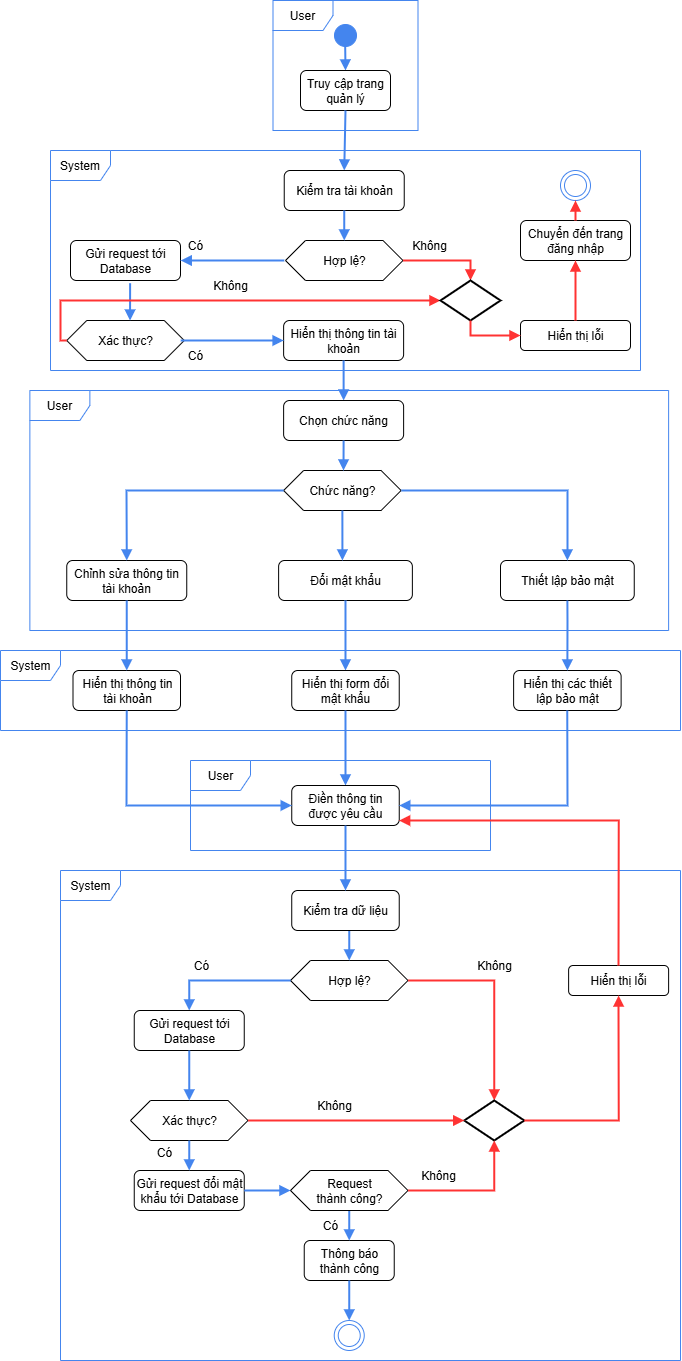
\includegraphics[width=0.6\textwidth]{Images/account-management_activity.png}
		      \caption{Activity Diagram - Account Management}
	      \end{figure}
	\item \textbf{UI:}


\end{itemize}
% Quản lý danh sách nhạc - Người dùng
\subsection{Quản lý danh sách nhạc - Playlist Management}
\begin{itemize}
	\item \textbf{Sequence Diagram:}
	      \begin{figure}[H]
		      \centering
		      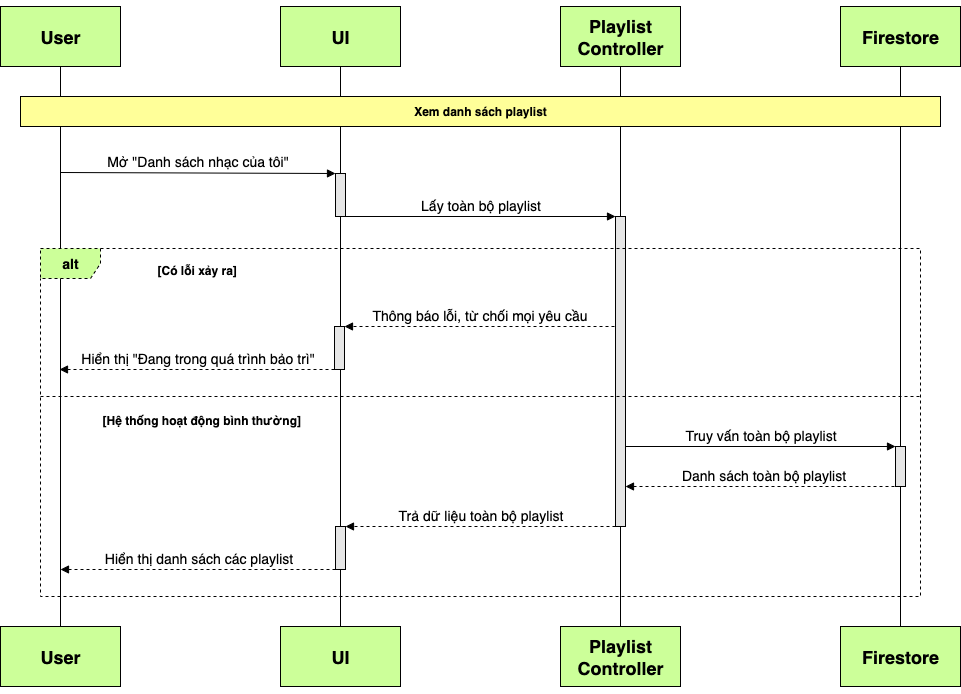
\includegraphics[width=0.9\textwidth]{Images/playlist/playlist-1_sd.png}
		      \caption{Sequence Diagram - Playlist Management (Access "My Playlist")}
	      \end{figure}
        \begin{figure}[H]
		      \centering
		      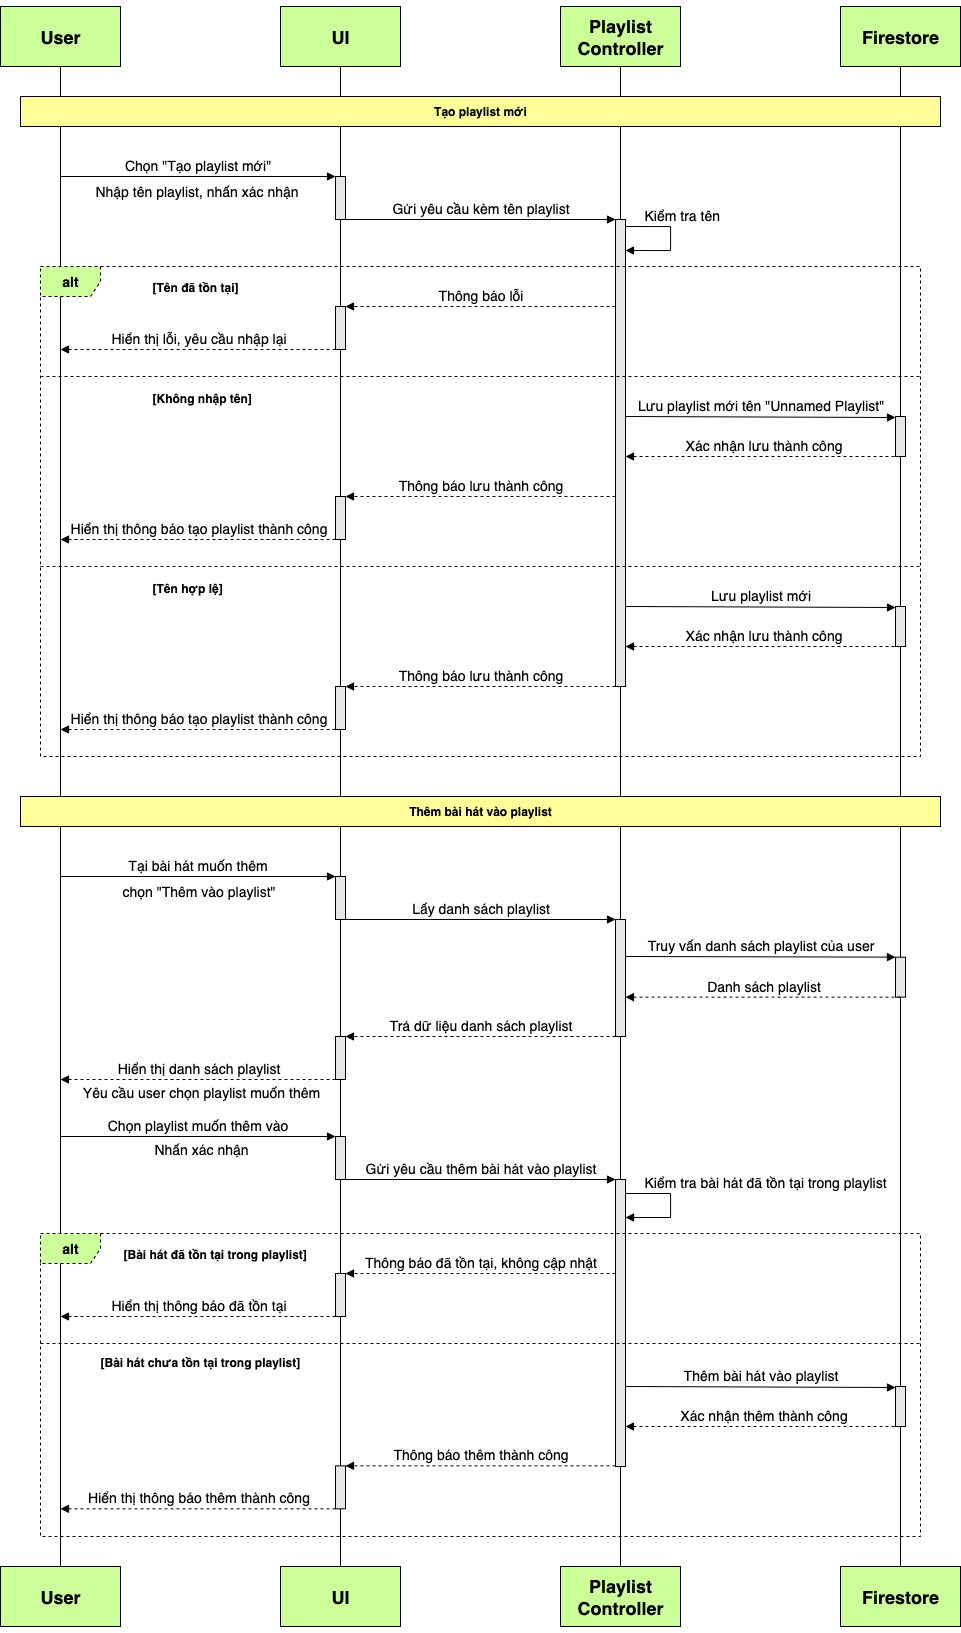
\includegraphics[width=0.8\textwidth]{Images/playlist/playlist-3ab_sd.png}
		      \caption{Sequence Diagram - Playlist Management (Create Playlist \& Add Song To Playlist)}
	      \end{figure}
        \begin{figure}[H]
		      \centering
		      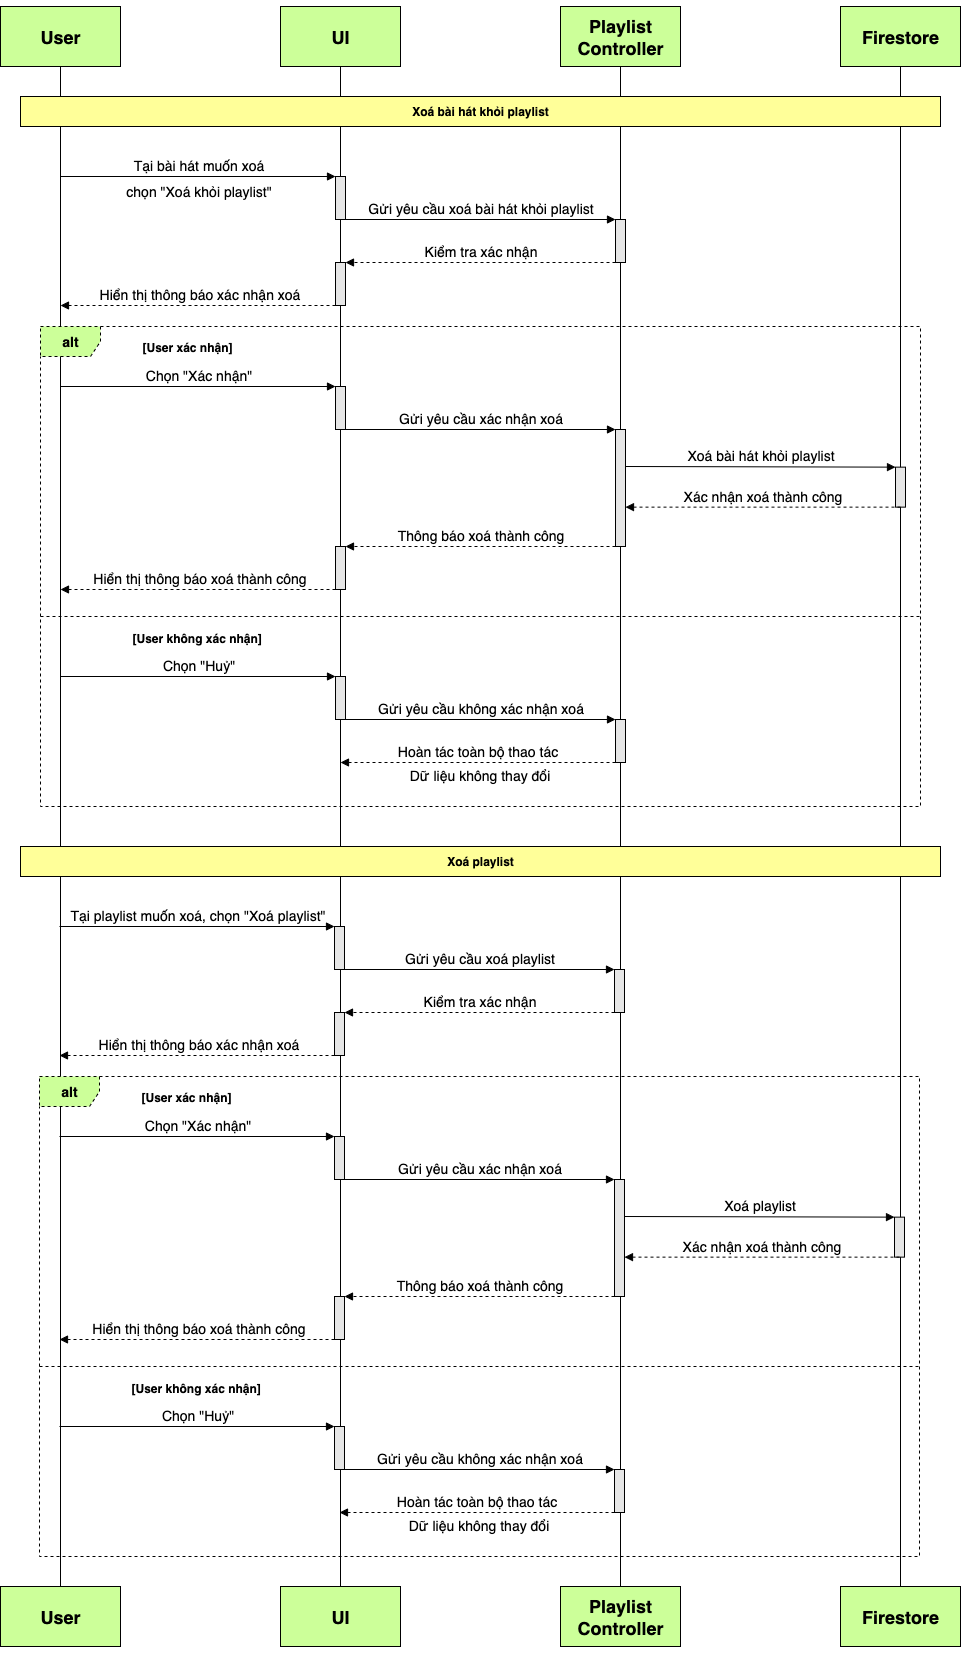
\includegraphics[width=0.8\textwidth]{Images/playlist/playlist-3cd_sd.png}
		      \caption{Sequence Diagram - Playlist Management (Remove Song From Playlist \& Delete Playlist)}
	      \end{figure}
	\item \textbf{Mục đích:} Thể hiện quy trình người dùng xem và thực hiện các thao tác điều khiển, quản lý danh sách nhạc (playlist) cá nhân của người dùng: truy cập "Danh sách nhạc của tôi", tạo playlist mới, thêm bài hát vào playlist, xoá bài hát khỏi playlist và xóa playlist.
	\item \textbf{Thành phần liên quan:}
	      \begin{itemize}
		      \item Người dùng (User): người thực hiện các thao tác quản lý playlist.
		      \item Giao diện quản lý (Management UI): giao diện để người dùng thao tác, nhập thông tin và hiển thị thông báo/kết quả.
		      \item Hệ thống xử lý (Playlist Controller): nhận thông tin và xử lý xác thực dữ liệu.
		      \item Cơ sở dữ liệu người dùng (Firestore): lưu trữ thông tin playlist của tài khoản người dùng.
	      \end{itemize}
	\item \textbf{Luồng tương tác:}
	      \begin{enumerate}
		      \item Người dùng truy cập "Danh sách nhạc của tôi".
          \item Nếu có lỗi xảy ra (mất kết nối máy chủ, hệ thống bận,...), hệ thống từ chối mọi yêu cầu từ người dùng và giao diện hiển thị thông báo "Đang trong quá trình bảo trì".
		      \item Nếu hệ thống hoạt động bình thường, hệ thống xử lý gửi yêu cầu đến cơ sở dữ liệu, cơ sở dữ liệu phản hồi kết quả là danh sách nhạc của người dùng hiện tại và hiển thị lên giao diện.
		      \item Người dụng thực hiện thao tác điều khiển:
		            \begin{itemize}
			            \item Nếu người dùng muốn tạo playlist mới:
			                  \begin{itemize}
				                  \item Người dùng chọn "Tạo playlist mới" trên giao diện, nhập tên playlist (có thể để trống) và nhấn xác nhận.
				                  \item Hệ thống tiếp nhận yêu cầu và kiểm tra tên playlist.
				                  \item Nếu tên đã tồn tại, hệ thống thông báo lỗi và yêu cầu người dùng nhập lại.
				                  \item Nếu người dùng không nhập tên cho playlist mà trực tiếp xác nhận, hệ thống sẽ tự động đặt tên theo định dạng mặc định "Unnamed Playlist" và lưu vào cơ sở dữ liệu.
				                  \item Nếu tên hợp lệ, hệ thống gửi yêu cầu tạo playlist mới đến cơ sở dữ liệu, cơ sở dữ liệu lưu trữ playlist mới và phản hồi kết quả.
				                  \item Giao diện hiển thị thông báo tạo playlist mới thành công và cập nhật theo dữ liệu mới.
			                  \end{itemize}
			            \item Nếu người dùng muốn thêm bài hát vào playlist:
			                  \begin{itemize}
				                  \item Người dùng chọn "Thêm vào playlist" với bài hát muốn thêm.
				                  \item Hệ thống tiếp nhận yêu cầu và truy vấn đến cơ sở dữ liệu để hiển thị danh sách playlist hiện có để người dùng chọn.
				                  \item Người dùng chọn playlist muốn thêm bài hát vào và nhấn xác nhận.
				                  \item Hệ thống tiếp nhận yêu cầu và kiểm tra bài hát đã tồn tại trong playlist hay chưa.
                          \item Nếu bài hát đã tồn tại trong playlist, hệ thống hiển thị thông báo đã tồn tại và không cập nhật bài hát.
                          \item Nếu bài hát chưa tồn tại trong playlist, hệ thống gửi yêu cầu thêm bài hát vào playlist đến cơ sở dữ liệu.
				                  \item Cơ sở dữ liệu thêm bài hát vào playlist và phản hồi kết quả.
				                  \item Giao diện hiển thị thông báo thêm thành công và cập nhật theo dữ liệu mới.
			                  \end{itemize}
			            \item Nếu người dùng muốn xoá bài hát khỏi playlist:
			                  \begin{itemize}
				                  \item Người dùng chọn "Xoá khỏi playlist" với bài hát muốn xoá.
                          \item Hệ thống hiển thị thông báo xác nhận xoá bài hát.
                          \item Nếu người dùng xác nhận xoá bài hát, hệ thống tiếp nhận và gửi yêu cầu đến cơ sở dữ liệu, cơ sở dữ liệu sẽ xoá bài hát khỏi playlist và phản hồi kết quả, giao diện hiển thị thông báo xoá thành công và cập nhật theo dữ liệu mới.
                          \item Nếu người dùng không xác nhận xoá bài hát mà chọn "Huỷ", hệ thống hoàn tác toàn bộ thao tác và cập nhật lại trạng thái ban đầu của danh sách playlist, dữ liệu không thay đổi.
			                  \end{itemize}
                  \item Nếu người dùng muốn xoá playlist:
                        \begin{itemize}
                          \item Người dùng chọn "Xoá playlist" tại playlist muốn xoá.
                          \item Hệ thống hiển thị thông báo xác nhận xoá playlist.
                          \item Nếu người dùng xác nhận xoá playlist, hệ thống tiếp nhận và gửi yêu cầu đến cơ sở dữ liệu, cơ sở dữ liệu sẽ xoá playlist và phản hồi kết quả, giao diện hiển thị thông báo xoá thành công và cập nhật theo dữ liệu mới.
                          \item Nếu người dùng không xác nhận xoá playlist mà chọn "Huỷ", hệ thống hoàn tác toàn bộ thao tác và cập nhật lại trạng thái ban đầu của danh sách playlist, dữ liệu không thay đổi.
                        \end{itemize}
		            \end{itemize}
            \item Hệ thống ghi nhận, cập nhật danh sách playlist của người dùng và làm mới UI.
	      \end{enumerate}

	\item \textbf{Activity Diagram:}
	      \begin{figure}[H]
			\centering
          	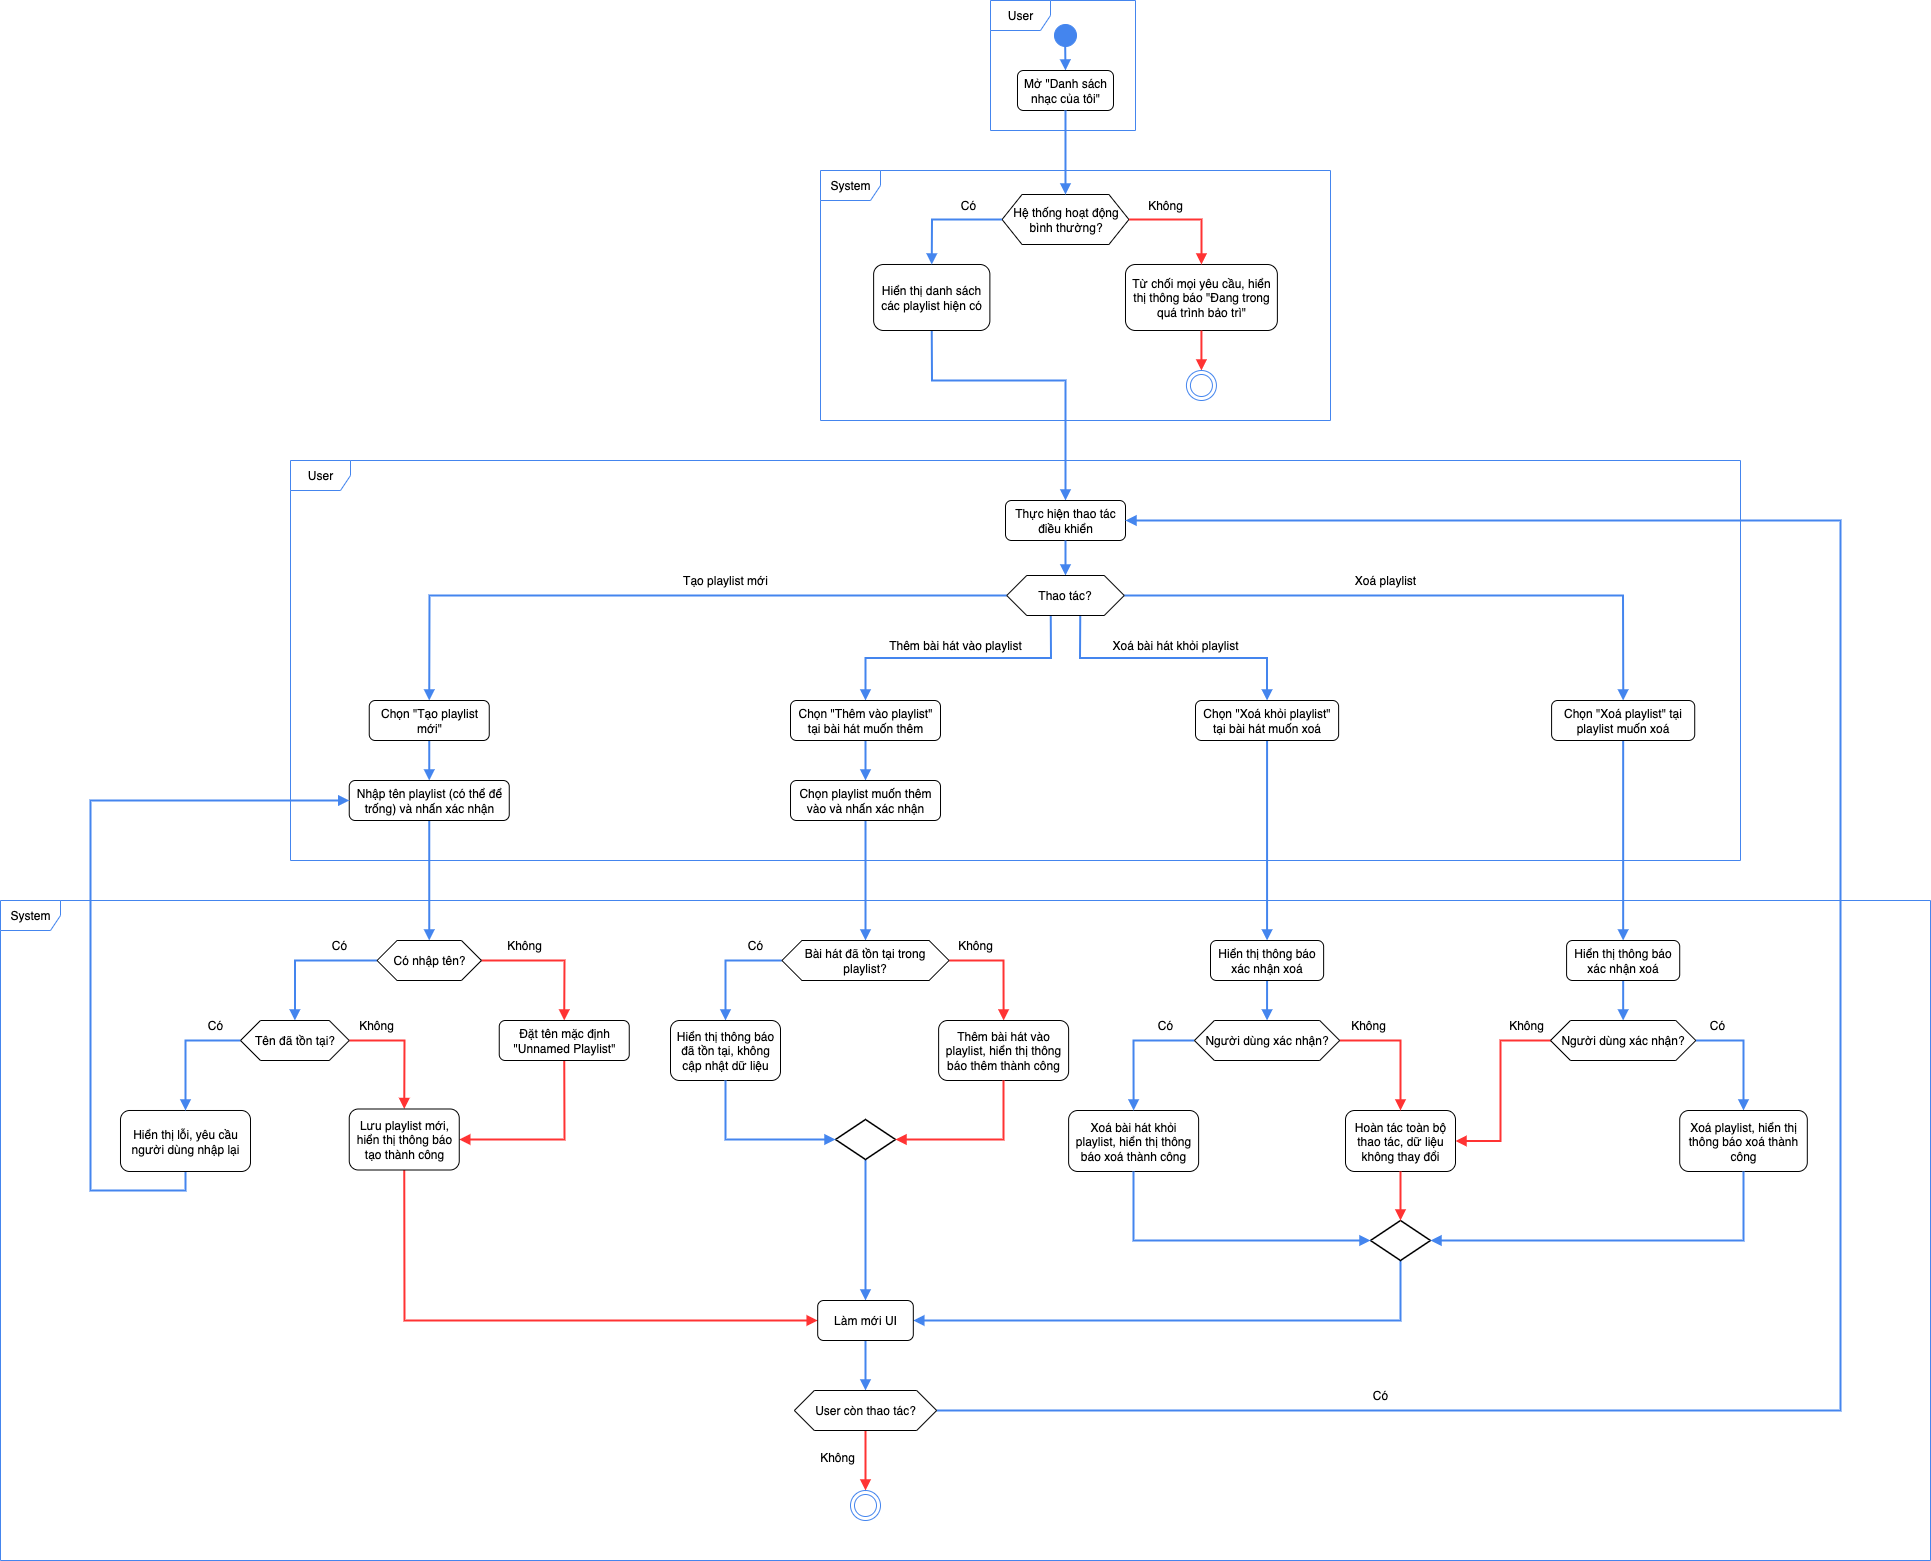
\includegraphics[width=1.0\textwidth, height=0.7\textheight]{Images/playlist/playlist-activity.png}
			\caption{Activity Diagram - Playlist Management}
	      \end{figure}
	\item \textbf{UI:}
\end{itemize}
% Khám phá và tìm kiếm - Người dùng, Nghệ sĩ
\subsection{Khám phá và tìm kiếm - Discovery \& Search}
\begin{itemize}
	\item \textbf{Sequence Diagram:}
	      \begin{figure}[H]
				\centering
				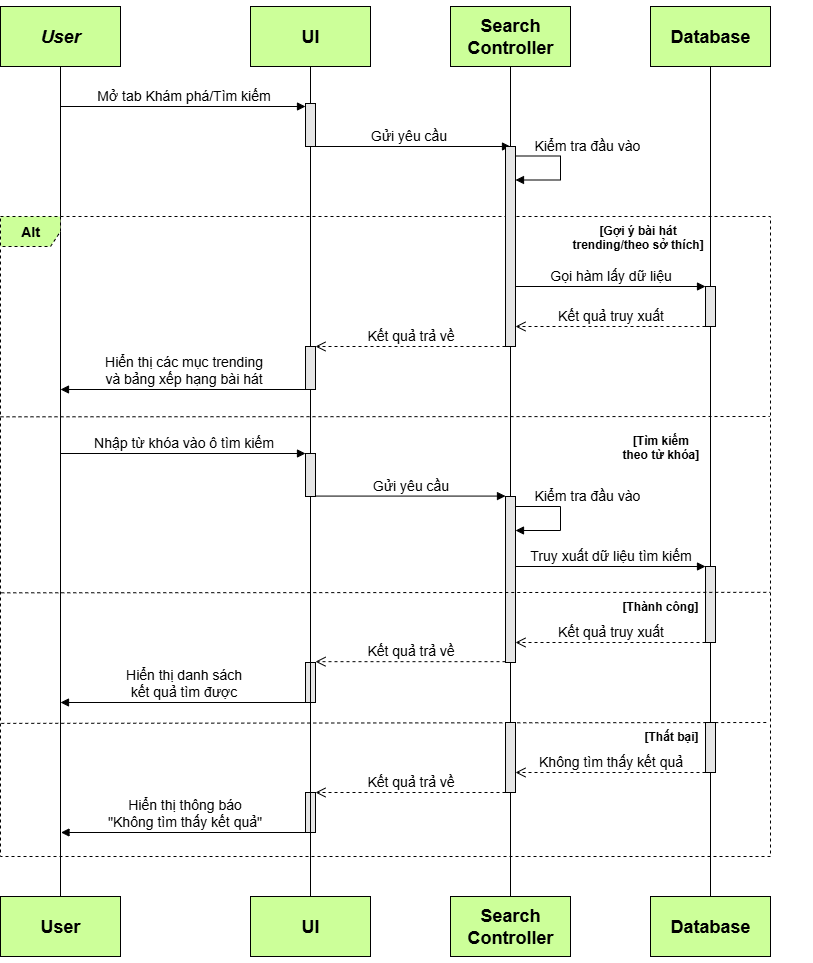
\includegraphics[width=0.9\textwidth, height=0.7\textheight]{Images/discover-search_sequence.png}
				\caption{Sequence Diagram - Discovery \& Search}
	      \end{figure}
	\item \textbf{Mục đích:} Thể hiện quy trình người dùng truy cập tính năng Khám phá/Tìm kiếm, bao gồm việc nhập từ khóa, nhận gợi ý cá nhân hóa, xem xu hướng (Trending/Top Chart), và kết quả trả về từ hệ thống.
	\item \textbf{Thành phần liên quan:}
	      \begin{itemize}
		      \item Người dùng (User): thực hiện thao tác mở tab khám phá/tìm kiếm, nhập từ khóa hoặc xem gợi ý.
		      \item Giao diện người dùng (UI): nơi hiển thị ô tìm kiếm, gợi ý, kết quả tìm kiếm hoặc bảng xếp hạng.
		      \item Search Controller: xử lý yêu cầu tìm kiếm, kiểm tra dữ liệu đầu vào và gọi truy vấn dữ liệu.
		      \item Database: lưu trữ dữ liệu bài hát, nghệ sĩ, album, playlist, lịch sử nghe để phục vụ tìm kiếm và gợi ý.
	      \end{itemize}
	\item \textbf{Luồng tương tác:}
	      \begin{enumerate}
			\item Người dùng mở tab \textbf{Khám phá/Tìm kiếm}.
			\item UI gửi yêu cầu đến Search Controller để lấy dữ liệu.
			\item Search Controller kiểm tra yêu cầu, gọi dữ liệu từ Database.
			\item Database trả kết quả: danh sách nhạc trending, top chart hoặc gợi ý theo sở thích.
			\item Người dùng nhập từ khóa (bài hát/album/nghệ sĩ/playlist).
			\item UI gửi yêu cầu tìm kiếm đến Search Controller.
			\item Search Controller kiểm tra dữ liệu, truy xuất Database.
			\item Database trả về kết quả:
			\begin{itemize}
				\item Nếu thành công $\rightarrow$ danh sách kết quả tìm thấy.
				\item Nếu thất bại $\rightarrow$ trả về thông báo “Không tìm thấy kết quả”.
			\end{itemize}
			\item UI hiển thị kết quả hoặc thông báo lỗi cho người dùng.
		  \end{enumerate}
	\item \textbf{Activity Diagram:}
		\begin{figure}[H]
				\centering
				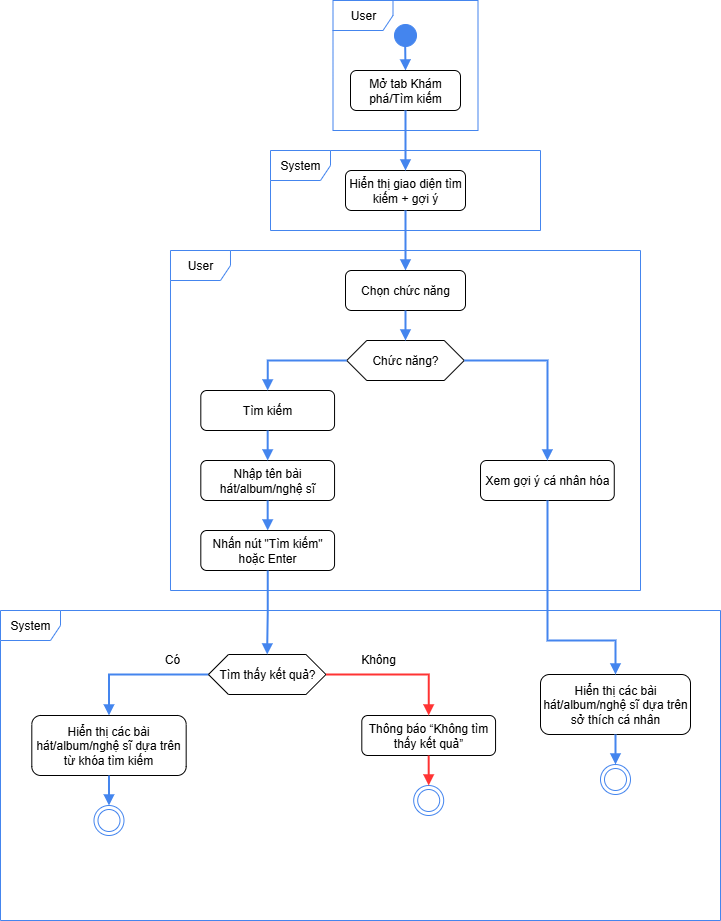
\includegraphics[width=0.9\textwidth]{Images/discover-search_activity.png}
				\caption{Activity Diagram - Discovery \& Search}
	      \end{figure}
	\item \textbf{UI:}
\end{itemize}

\end{document}